\documentclass[aspectratio=169,10pt]{beamer}

\usetheme{default}
\usecolortheme{default}
\setbeamertemplate{navigation symbols}{}
\setbeamersize{text margin left=0.50cm, text margin right=0.50cm}

\usepackage[utf8]{inputenc}
\usepackage[T1]{fontenc}
\usepackage[english]{babel}
\usepackage{booktabs}
\usepackage{array}
\usepackage{tikz}
\usetikzlibrary{arrows.meta,positioning,shapes.geometric,calc,fit,backgrounds}

% --- Color Palette (Modern Engineering Look) ---
\definecolor{aaaNavy}{RGB}{18, 48, 89}
\definecolor{aaaBlue}{RGB}{33, 92, 160}
\definecolor{aaaTeal}{RGB}{0, 132, 118}
\definecolor{aaaGreen}{RGB}{24, 130, 62}
\definecolor{aaaAmber}{RGB}{204, 88, 0}
\definecolor{aaaRed}{RGB}{185, 38, 38}
\definecolor{aaaSlate}{RGB}{72, 85, 102}
\definecolor{aaaLightBg}{RGB}{244, 247, 251}
\definecolor{aaaBorder}{RGB}{205, 214, 226}

\setbeamercolor{normal text}{fg=aaaNavy!92!black, bg=white}
\setbeamercolor{structure}{fg=aaaNavy}

% --- Edge-to-Edge Frame Title ---
\setbeamertemplate{frametitle}{%
  \nointerlineskip%
  \begin{beamercolorbox}[wd=\paperwidth,ht=0.78cm,dp=0.20cm,leftskip=0.55cm,rightskip=0.55cm]{frametitle}%
    \begin{tikzpicture}[remember picture, overlay]
      \fill[aaaNavy] (current page.north west) rectangle ([yshift=-0.98cm]current page.north east);
      \fill[aaaTeal] ([yshift=-0.98cm]current page.north west) rectangle ([yshift=-1.04cm]current page.north east);
    \end{tikzpicture}%
    \vbox to 0.78cm{\vfil\hbox{\fontsize{12}{14.5}\selectfont\bfseries\color{white}\insertframetitle}\vfil}%
  \end{beamercolorbox}%
  \vspace{-0.10cm}%
}

% --- Clean Footline ---
\setbeamertemplate{footline}{%
  \hbox{%
    \begin{beamercolorbox}[wd=\paperwidth,ht=0.38cm,dp=0.12cm,leftskip=0.55cm,rightskip=0.55cm]{footline}%
      \tiny\color{aaaSlate}%
      \textbf{Agile Agentic ASPICE (AAA)} \quad|\quad Architecture \& Process Blueprint (\texttt{aTrainingTracker})%
      \hfill%
      \textbf{Slide \insertframenumber{} / \inserttotalframenumber}%
    \end{beamercolorbox}%
  }%
}

% --- Reusable Banner Styles ---
\tikzset{
  bannerNavy/.style={
    rectangle, rounded corners=3.5pt, draw=aaaNavy, line width=0.85pt,
    fill=aaaNavy!7, inner xsep=8pt, inner ysep=5pt, align=left
  },
  bannerAmber/.style={
    rectangle, rounded corners=3.5pt, draw=aaaAmber, line width=0.85pt,
    fill=aaaAmber!8, inner xsep=8pt, inner ysep=5pt, align=left
  },
  bannerGreen/.style={
    rectangle, rounded corners=3.5pt, draw=aaaGreen, line width=0.85pt,
    fill=aaaGreen!8, inner xsep=8pt, inner ysep=5pt, align=left
  }
}

\newcommand{\bitem}{\textcolor{aaaTeal}{$\bullet$}\ }

\begin{document}

% =========================================================================
% SLIDE 1: TITLE
% =========================================================================
\begin{frame}[plain]
  \begin{tikzpicture}[remember picture, overlay]
    % Background header & body
    \fill[aaaNavy] (current page.north west) rectangle ([yshift=-4.45cm]current page.north east);
    \fill[aaaTeal] ([yshift=-4.45cm]current page.north west) rectangle ([yshift=-4.57cm]current page.north east);
    \fill[aaaLightBg] ([yshift=-4.57cm]current page.north west) rectangle (current page.south east);

    % Title text in Navy header
    \node[anchor=west, text=white, font=\fontsize{20.74}{25}\selectfont\bfseries]
      at ([xshift=0.85cm, yshift=-1.55cm]current page.north west)
      {Agile Agentic ASPICE (AAA)};
    \node[anchor=west, text=aaaTeal!30!white, font=\normalsize\bfseries]
      at ([xshift=0.85cm, yshift=-2.45cm]current page.north west)
      {From ``Vibe Coding'' to an Autonomous, Control-Loop-Governed AI Software Factory};
    \node[anchor=west, text=white!85, font=\footnotesize]
      at ([xshift=0.85cm, yshift=-3.35cm]current page.north west)
      {Scrum Sprints $\cdot$ 5 ASPICE Stages $\cdot$ Independent Quality Gates $\cdot$ 3-Loop Cascade Control};

    % 3 Summary highlight boxes in lower area
    \node[rectangle, rounded corners=4pt, fill=white, draw=aaaBorder, line width=0.85pt,
          text width=4.15cm, minimum height=2.25cm, anchor=north west, align=left, inner sep=7pt]
      at ([xshift=0.85cm, yshift=-5.15cm]current page.north west) {
        \textcolor{aaaNavy}{\footnotesize\bfseries 1. Process Guardrails}\\[3pt]
        \scriptsize\color{aaaSlate}
        5 coupled ASPICE stages with independent \textbf{Quality Gates} prevent shortcuts, scope creep, and untested code.
      };

    \node[rectangle, rounded corners=4pt, fill=white, draw=aaaBorder, line width=0.85pt,
          text width=4.15cm, minimum height=2.25cm, anchor=north west, align=left, inner sep=7pt]
      at ([xshift=5.72cm, yshift=-5.15cm]current page.north west) {
        \textcolor{aaaTeal}{\footnotesize\bfseries 2. Cascade Control}\\[3pt]
        \scriptsize\color{aaaSlate}
        Fast inner feedback loops (compiler, tests, gatekeeper \texttt{agent2}) reject hallucinations and drift \textbf{before} human review.
      };

    \node[rectangle, rounded corners=4pt, fill=white, draw=aaaBorder, line width=0.85pt,
          text width=4.15cm, minimum height=2.25cm, anchor=north west, align=left, inner sep=7pt]
      at ([xshift=10.59cm, yshift=-5.15cm]current page.north west) {
        \textcolor{aaaAmber}{\footnotesize\bfseries 3. Time Leverage}\\[3pt]
        \scriptsize\color{aaaSlate}
        Only \textbf{2--3h of focused human time} per sprint instead of constant 15-minute wait loops. Agents work \textbf{up to 24h/day}.
      };

    % Author / Date footer
    \node[anchor=south west, font=\scriptsize\bfseries, text=aaaNavy]
      at ([xshift=0.85cm, yshift=0.50cm]current page.south west)
      {Rainer Blind \quad\normalfont\scriptsize\color{aaaSlate}| \quad Architecture \& Process Blueprint (\texttt{aTrainingTracker})};
    \node[anchor=south east, font=\scriptsize\bfseries, text=aaaSlate]
      at ([xshift=-0.85cm, yshift=0.50cm]current page.south east)
      {\today};
  \end{tikzpicture}
\end{frame}

% =========================================================================
% SLIDE 2: THE 3 PILLARS (WHY TRIPLE-A?)
% =========================================================================
\begin{frame}{The Core Idea: Why \textbf{AAA} (\emph{Agile Agentic ASPICE})?}
  \centering
  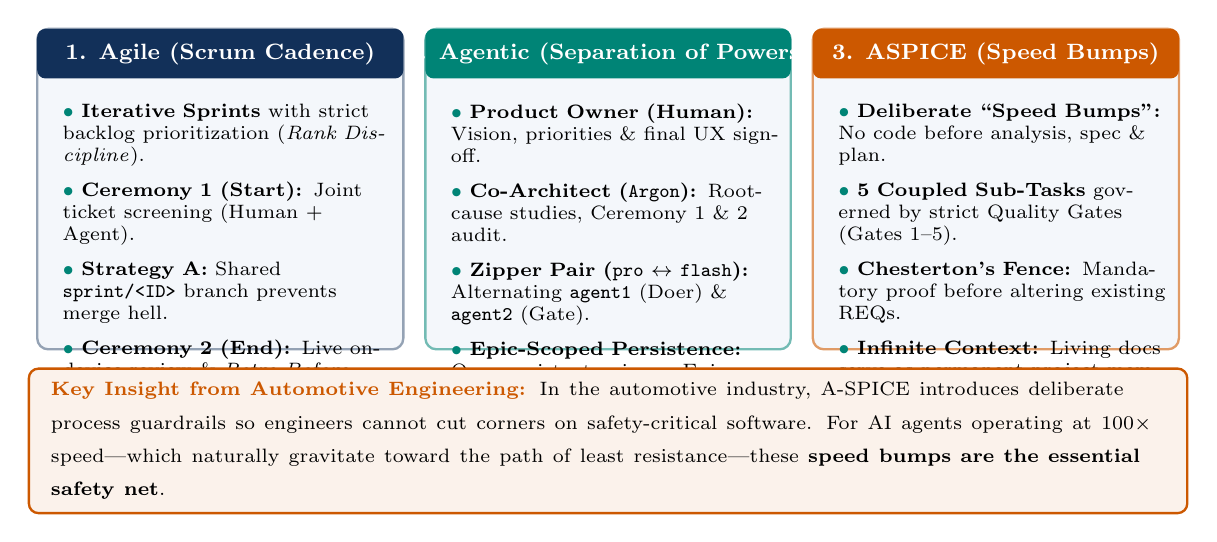
\begin{tikzpicture}[x=1cm, y=1cm]
    % Column 1: AGILE
    \draw[fill=aaaLightBg, draw=aaaNavy!45, line width=0.85pt, rounded corners=4pt] (-7.25, -1.52) rectangle (-2.60, 2.55);
    \fill[aaaNavy, rounded corners=3pt] (-7.25, 1.92) rectangle (-2.60, 2.55);
    \node[font=\footnotesize\bfseries, text=white] at (-4.925, 2.23) {1. \textbf{A}gile (Scrum Cadence)};
    \node[anchor=north west, text width=4.30cm, font=\scriptsize] at (-7.05, 1.72) {
      \bitem \textbf{Iterative Sprints} with strict backlog prioritization (\emph{Rank Discipline}).\\[4.5pt]
      \bitem \textbf{Ceremony 1 (Start):} Joint ticket screening (Human + Agent).\\[4.5pt]
      \bitem \textbf{Strategy A:} Shared \texttt{sprint/<ID>} branch prevents merge hell.\\[4.5pt]
      \bitem \textbf{Ceremony 2 (End):} Live on-device review \& \emph{Retro Before Merge}.
    };

    % Column 2: AGENTIC
    \draw[fill=aaaLightBg, draw=aaaTeal!55, line width=0.85pt, rounded corners=4pt] (-2.32, -1.52) rectangle (2.32, 2.55);
    \fill[aaaTeal, rounded corners=3pt] (-2.32, 1.92) rectangle (2.32, 2.55);
    \node[font=\footnotesize\bfseries, text=white] at (0.0, 2.23) {2. \textbf{A}gentic (Separation of Powers)};
    \node[anchor=north west, text width=4.30cm, font=\scriptsize] at (-2.12, 1.72) {
      \bitem \textbf{Product Owner (Human):} Vision, priorities \& final UX sign-off.\\[4.5pt]
      \bitem \textbf{Co-Architect (\texttt{Argon}):} Root-cause studies, Ceremony 1 \& 2 audit.\\[4.5pt]
      \bitem \textbf{Zipper Pair (\texttt{pro} $\leftrightarrow$ \texttt{flash}):} Alternating \texttt{agent1} (Doer) \& \texttt{agent2} (Gate).\\[4.5pt]
      \bitem \textbf{Epic-Scoped Persistence:} One persistent pair per Epic across the sprint.
    };

    % Column 3: ASPICE
    \draw[fill=aaaLightBg, draw=aaaAmber!60, line width=0.85pt, rounded corners=4pt] (2.60, -1.52) rectangle (7.25, 2.55);
    \fill[aaaAmber, rounded corners=3pt] (2.60, 1.92) rectangle (7.25, 2.55);
    \node[font=\footnotesize\bfseries, text=white] at (4.925, 2.23) {3. \textbf{A}SPICE (Speed Bumps)};
    \node[anchor=north west, text width=4.30cm, font=\scriptsize] at (2.80, 1.72) {
      \bitem \textbf{Deliberate ``Speed Bumps'':} No code before analysis, spec \& plan.\\[4.5pt]
      \bitem \textbf{5 Coupled Sub-Tasks} governed by strict Quality Gates (Gates 1--5).\\[4.5pt]
      \bitem \textbf{Chesterton's Fence:} Mandatory proof before altering existing REQs.\\[4.5pt]
      \bitem \textbf{Infinite Context:} Living docs serve as permanent project memory.
    };

    % Bottom Takeaway Banner
    \node[bannerAmber, text width=14.15cm, anchor=north] at (0, -1.75) {
      \scriptsize\textcolor{aaaAmber}{\textbf{Key Insight from Automotive Engineering:}}
      In the automotive industry, A-SPICE introduces deliberate process guardrails so engineers cannot cut corners on safety-critical software.
      For AI agents operating at 100$\times$ speed—which naturally gravitate toward the path of least resistance—these \textbf{speed bumps are the essential safety net}.
    };
  \end{tikzpicture}
\end{frame}

% =========================================================================
% SLIDE 3: WORKFLOW 1 — THE HYBRID V-MODEL
% =========================================================================
\begin{frame}{Workflow 1: The Hybrid V-Model (Human \& Argon $\leftrightarrow$ Autonomous Pipeline)}
  \centering
  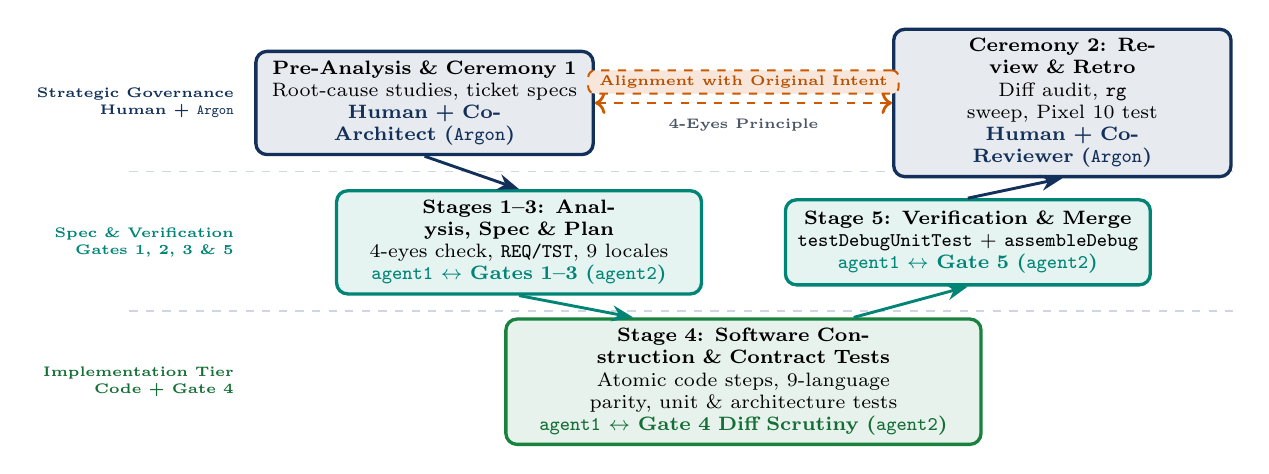
\begin{tikzpicture}[
    x=1cm, y=1cm,
    topBox/.style={rectangle, rounded corners=4pt, draw=aaaNavy, very thick, fill=aaaNavy!10, text width=4.05cm, align=center, minimum height=1.18cm, font=\scriptsize},
    midBox/.style={rectangle, rounded corners=4pt, draw=aaaTeal, very thick, fill=aaaTeal!10, text width=4.40cm, align=center, minimum height=1.08cm, font=\scriptsize},
    botBox/.style={rectangle, rounded corners=4pt, draw=aaaGreen, very thick, fill=aaaGreen!10, text width=5.80cm, align=center, minimum height=1.12cm, font=\scriptsize},
    badge/.style={rectangle, rounded corners=2.5pt, fill=aaaAmber!15, draw=aaaAmber, line width=0.7pt, font=\tiny\bfseries, text=aaaAmber!90!black, inner xsep=4pt, inner ysep=2pt},
    arr/.style={-{Stealth[scale=1.0]}, line width=1.05pt, draw=aaaNavy}
  ]
    % V-Model tier labels on left
    \node[anchor=east, font=\tiny\bfseries, text=aaaNavy, align=right] at (-5.65, 2.02) {Strategic Governance\\Human + \texttt{Argon}};
    \node[anchor=east, font=\tiny\bfseries, text=aaaTeal, align=right] at (-5.65, 0.25) {Spec \& Verification\\Gates 1, 2, 3 \& 5};
    \node[anchor=east, font=\tiny\bfseries, text=aaaGreen!85!black, align=right] at (-5.65, -1.52) {Implementation Tier\\Code + Gate 4};

    \draw[dashed, draw=aaaBorder, line width=0.7pt] (-7.10, 1.15) -- (7.00, 1.15);
    \draw[dashed, draw=aaaBorder, line width=0.7pt] (-7.10, -0.62) -- (7.00, -0.62);

    % Top left & right (Human + Argon)
    \node[topBox] (leftTop) at (-3.35, 2.02)
      {\textbf{Pre-Analysis \& Ceremony 1}\\Root-cause studies, ticket specs\\\textcolor{aaaNavy}{\textbf{Human + Co-Architect (\texttt{Argon})}}};
    \node[topBox] (rightTop) at (4.75, 2.02)
      {\textbf{Ceremony 2: Review \& Retro}\\Diff audit, \texttt{rg} sweep, Pixel 10 test\\\textcolor{aaaNavy}{\textbf{Human + Co-Reviewer (\texttt{Argon})}}};

    % Middle left & right (Stages 1-3 and Stage 5, strictly 3 lines each!)
    \node[midBox] (midLeft) at (-2.15, 0.25)
      {\textbf{Stages 1--3: Analysis, Spec \& Plan}\\4-eyes check, \texttt{REQ/TST}, 9 locales\\\textcolor{aaaTeal}{\textbf{\texttt{agent1} $\leftrightarrow$ Gates 1--3 (\texttt{agent2})}}};
    \node[midBox] (midRight) at (3.55, 0.25)
      {\textbf{Stage 5: Verification \& Merge}\\\texttt{testDebugUnitTest} + \texttt{assembleDebug}\\\textcolor{aaaTeal}{\textbf{\texttt{agent1} $\leftrightarrow$ Gate 5 (\texttt{agent2})}}};

    % Bottom (Stage 4 Implementation)
    \node[botBox] (bottom) at (0.70, -1.52)
      {\textbf{Stage 4: Software Construction \& Contract Tests}\\Atomic code steps, 9-language parity, unit \& architecture tests\\\textcolor{aaaGreen!85!black}{\textbf{\texttt{agent1} $\leftrightarrow$ Gate 4 Diff Scrutiny (\texttt{agent2})}}};

    % Arrows along the V
    \draw[arr] (leftTop.south) -- (midLeft.north);
    \draw[arr, draw=aaaTeal] (midLeft.south) -- ([xshift=-1.4cm]bottom.north);
    \draw[arr, draw=aaaTeal] ([xshift=1.4cm]bottom.north) -- (midRight.south);
    \draw[arr] (midRight.north) -- (rightTop.south);

    % Horizontal Verification Arrow between leftTop and rightTop
    \draw[<->, dashed, line width=1.0pt, draw=aaaAmber] (leftTop.east) --
      node[badge, above=3pt] {Alignment with Original Intent}
      node[below=2pt, font=\tiny\bfseries, text=aaaSlate] {4-Eyes Principle}
      (rightTop.west);
  \end{tikzpicture}
\end{frame}

% =========================================================================
% SLIDE 4: WORKFLOW 2 — SCRUM SPRINT & GIT STRATEGY A
% =========================================================================
\begin{frame}{Workflow 2: The Scrum Sprint \& Git Branching Flow (Strategy A)}
  \centering
  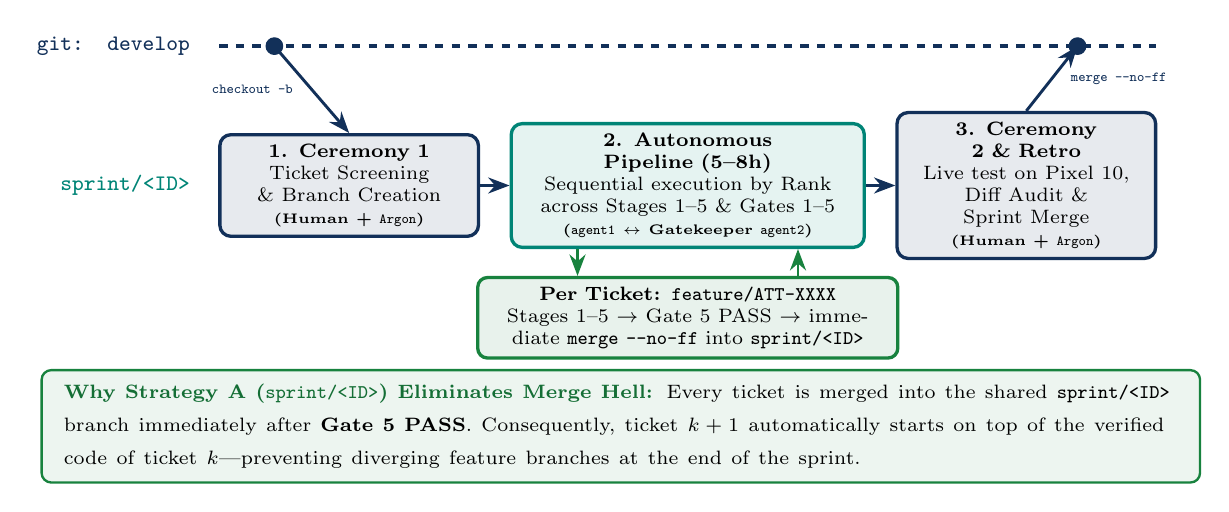
\begin{tikzpicture}[
    x=1cm, y=1cm,
    boxA/.style={rectangle, rounded corners=4pt, draw=aaaNavy, very thick, fill=aaaNavy!10, text width=3.05cm, align=center, minimum height=1.22cm, font=\scriptsize},
    boxF/.style={rectangle, rounded corners=4pt, draw=aaaTeal, very thick, fill=aaaTeal!10, text width=4.25cm, align=center, minimum height=1.22cm, font=\scriptsize},
    featBox/.style={rectangle, rounded corners=3.5pt, draw=aaaGreen, very thick, fill=aaaGreen!10, text width=5.10cm, align=center, minimum height=0.85cm, font=\scriptsize},
    arr/.style={-{Stealth[scale=1.0]}, line width=1.05pt, draw=aaaNavy}
  ]
    % Develop branch line
    \node[anchor=east, font=\footnotesize\bfseries, text=aaaNavy] at (-5.35, 2.15) {\texttt{git: develop}};
    \draw[dashed, line width=1.4pt, draw=aaaNavy] (-5.10, 2.15) -- (6.80, 2.15);
    \filldraw[aaaNavy] (-4.40, 2.15) circle (3.0pt);
    \filldraw[aaaNavy] (5.80, 2.15) circle (3.0pt);

    % Sprint branch label
    \node[anchor=east, font=\footnotesize\bfseries, text=aaaTeal] at (-5.35, 0.38) {\texttt{sprint/<ID>}};

    % 3 Main Sprint Phases
    \node[boxA] (c1) at (-3.45, 0.38)
      {\textbf{1. Ceremony 1}\\Ticket Screening\\\& Branch Creation\\{\tiny\textbf{(Human + \texttt{Argon})}}};

    \node[boxF] (p2) at (0.85, 0.38)
      {\textbf{2. Autonomous Pipeline (5--8h)}\\Sequential execution by Rank\\across Stages 1--5 \& Gates 1--5\\{\tiny\textbf{(\texttt{agent1} $\leftrightarrow$ Gatekeeper \texttt{agent2})}}};

    \node[boxA] (c2) at (5.15, 0.38)
      {\textbf{3. Ceremony 2 \& Retro}\\Live test on Pixel 10,\\Diff Audit \& Sprint Merge\\{\tiny\textbf{(Human + \texttt{Argon})}}};

    % Feature branch loop below Phase 2
    \node[featBox] (fb) at (0.85, -1.30)
      {\textbf{Per Ticket: \texttt{feature/ATT-XXXX}}\\Stages 1--5 $\rightarrow$ Gate 5 PASS $\rightarrow$ immediate \texttt{merge --no-ff} into \texttt{sprint/<ID>}};

    % Branching & phase arrows
    \draw[arr] (-4.40, 2.15) -- node[left=3pt, font=\tiny\bfseries, text=aaaNavy] {\texttt{checkout -b}} (c1.north);
    \draw[arr] (c1.east) -- (p2.west);
    \draw[arr] (p2.east) -- (c2.west);
    \draw[arr] (c2.north) -- node[right=3pt, font=\tiny\bfseries, text=aaaNavy] {\texttt{merge --no-ff}} (5.80, 2.15);

    \draw[arr, draw=aaaGreen] ([xshift=-1.4cm]p2.south) -- ([xshift=-1.4cm]fb.north);
    \draw[arr, draw=aaaGreen] ([xshift=1.4cm]fb.north) -- ([xshift=1.4cm]p2.south);

    % Bottom explanation banner
    \node[bannerGreen, text width=14.15cm, anchor=north] at (0, -1.95) {
      \scriptsize\textcolor{aaaGreen!85!black}{\textbf{Why Strategy A (\texttt{sprint/<ID>}) Eliminates Merge Hell:}}
      Every ticket is merged into the shared \texttt{sprint/<ID>} branch immediately after \textbf{Gate 5 PASS}. Consequently, ticket $k+1$ automatically starts on top of the verified code of ticket $k$—preventing diverging feature branches at the end of the sprint.
    };
  \end{tikzpicture}
\end{frame}

% =========================================================================
% SLIDE 5: WORKFLOW 3 — THE 2-TIER CASCADE (PARENT <-> 5 SUB-TASKS)
% =========================================================================
\begin{frame}{Workflow 3: The 2-Tier Cascade (Parent Ticket $\leftrightarrow$ 5 Stage Sub-Tasks)}
  \centering
  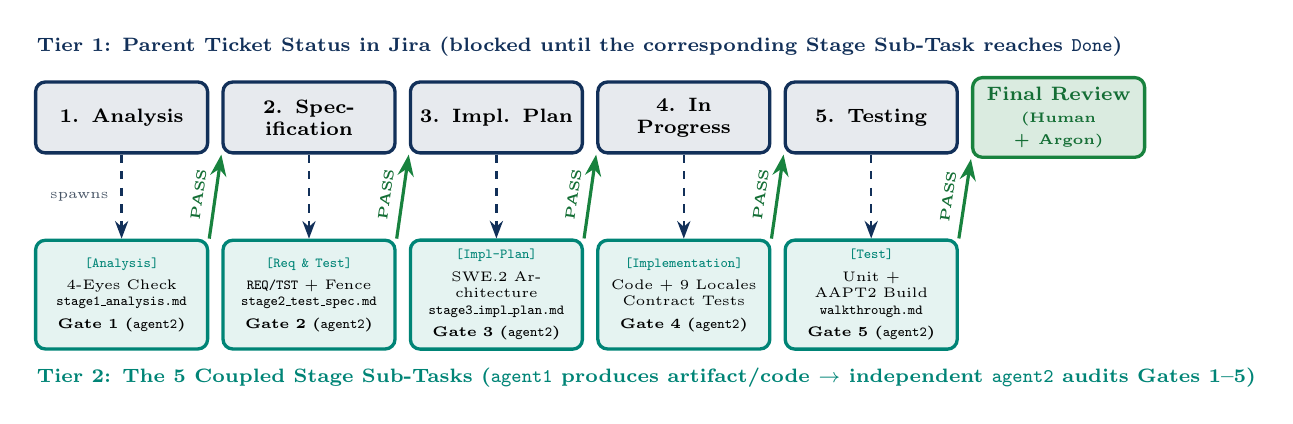
\begin{tikzpicture}[
    x=1cm, y=1cm,
    pBox/.style={rectangle, rounded corners=3.5pt, draw=aaaNavy, very thick, fill=aaaNavy!10, text width=1.95cm, align=center, minimum height=0.90cm, font=\scriptsize\bfseries},
    sBox/.style={rectangle, rounded corners=3.5pt, draw=aaaTeal, very thick, fill=aaaTeal!10, text width=1.95cm, align=center, minimum height=1.38cm, font=\tiny},
    spawnArr/.style={-{Stealth[scale=0.9]}, dashed, line width=0.9pt, draw=aaaNavy},
    passArr/.style={-{Stealth[scale=0.95]}, line width=1.15pt, draw=aaaGreen}
  ]
    % Level 1 Header
    \node[anchor=west, font=\scriptsize\bfseries, text=aaaNavy] at (-7.15, 2.35)
      {Tier 1: Parent Ticket Status in Jira (blocked until the corresponding Stage Sub-Task reaches \texttt{Done})};

    % Parent boxes (y = 1.45)
    \node[pBox] (p1) at (-5.95, 1.45) {1. Analysis};
    \node[pBox] (p2) at (-3.57, 1.45) {2. Specification};
    \node[pBox] (p3) at (-1.19, 1.45) {3. Impl. Plan};
    \node[pBox] (p4) at ( 1.19, 1.45) {4. In Progress};
    \node[pBox] (p5) at ( 3.57, 1.45) {5. Testing};
    \node[pBox, draw=aaaGreen, fill=aaaGreen!16, text=aaaGreen!85!black] (p6) at (5.95, 1.45)
      {Final Review\\{\tiny(Human + Argon)}};

    % Subtask boxes (y = -0.80)
    \node[sBox] (s1) at (-5.95, -0.80)
      {\textcolor{aaaTeal}{\textbf{\texttt{[Analysis]}}}\\[2pt]4-Eyes Check\\\texttt{stage1\_analysis.md}\\[2pt]\textbf{Gate 1 (\texttt{agent2})}};
    \node[sBox] (s2) at (-3.57, -0.80)
      {\textcolor{aaaTeal}{\textbf{\texttt{[Req \& Test]}}}\\[2pt]\texttt{REQ/TST} + Fence\\\texttt{stage2\_test\_spec.md}\\[2pt]\textbf{Gate 2 (\texttt{agent2})}};
    \node[sBox] (s3) at (-1.19, -0.80)
      {\textcolor{aaaTeal}{\textbf{\texttt{[Impl-Plan]}}}\\[2pt]SWE.2 Architecture\\\texttt{stage3\_impl\_plan.md}\\[2pt]\textbf{Gate 3 (\texttt{agent2})}};
    \node[sBox] (s4) at ( 1.19, -0.80)
      {\textcolor{aaaTeal}{\textbf{\texttt{[Implementation]}}}\\[2pt]Code + 9 Locales\\Contract Tests\\[2pt]\textbf{Gate 4 (\texttt{agent2})}};
    \node[sBox] (s5) at ( 3.57, -0.80)
      {\textcolor{aaaTeal}{\textbf{\texttt{[Test]}}}\\[2pt]Unit + AAPT2 Build\\\texttt{walkthrough.md}\\[2pt]\textbf{Gate 5 (\texttt{agent2})}};

    % Level 2 Header
    \node[anchor=west, font=\scriptsize\bfseries, text=aaaTeal] at (-7.15, -1.85)
      {Tier 2: The 5 Coupled Stage Sub-Tasks (\texttt{agent1} produces artifact/code $\rightarrow$ independent \texttt{agent2} audits Gates 1--5)};

    % Down arrows (spawn / block)
    \draw[spawnArr] (p1.south) -- node[left=1pt, font=\tiny, text=aaaSlate] {spawns} (s1.north);
    \draw[spawnArr] (p2.south) -- (s2.north);
    \draw[spawnArr] (p3.south) -- (s3.north);
    \draw[spawnArr] (p4.south) -- (s4.north);
    \draw[spawnArr] (p5.south) -- (s5.north);

    % Diagonal Gate PASS arrows advancing Parent to next stage
    \draw[passArr] (s1.north east) -- node[midway, sloped, above=0.5pt, font=\tiny\bfseries, text=aaaGreen!85!black] {PASS} (p2.south west);
    \draw[passArr] (s2.north east) -- node[midway, sloped, above=0.5pt, font=\tiny\bfseries, text=aaaGreen!85!black] {PASS} (p3.south west);
    \draw[passArr] (s3.north east) -- node[midway, sloped, above=0.5pt, font=\tiny\bfseries, text=aaaGreen!85!black] {PASS} (p4.south west);
    \draw[passArr] (s4.north east) -- node[midway, sloped, above=0.5pt, font=\tiny\bfseries, text=aaaGreen!85!black] {PASS} (p5.south west);
    \draw[passArr] (s5.north east) -- node[midway, sloped, above=0.5pt, font=\tiny\bfseries, text=aaaGreen!85!black] {PASS} (p6.south west);
  \end{tikzpicture}
\end{frame}

% =========================================================================
% SLIDE 6: WORKFLOW 4 — SUB-TASK STATE MACHINE
% =========================================================================
\begin{frame}{Workflow 4: The Sub-Task State Machine (incl.\ Revision \& Escalation)}
  \centering
  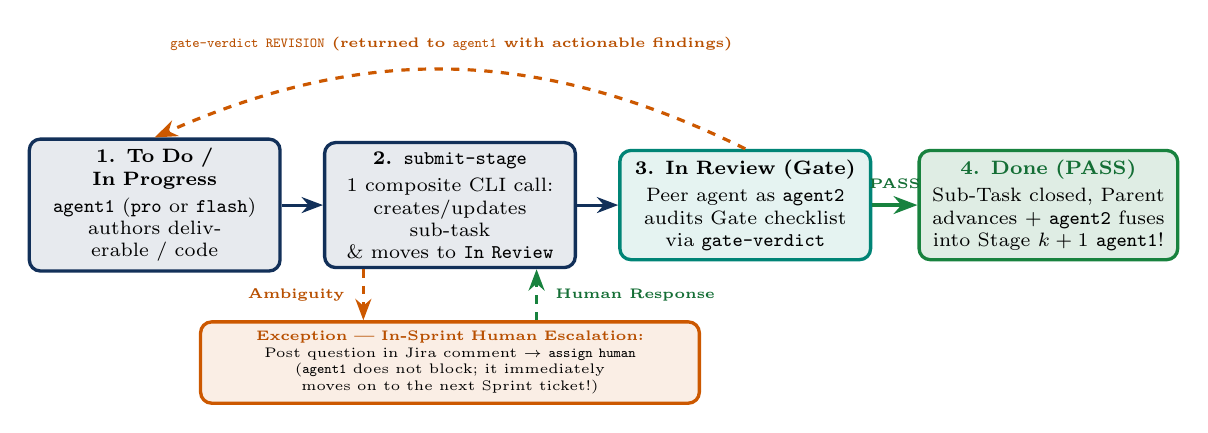
\begin{tikzpicture}[
    x=1cm, y=1cm,
    stateBox/.style={rectangle, rounded corners=4pt, draw=aaaNavy, very thick, fill=aaaNavy!10, text width=2.95cm, align=center, minimum height=1.32cm, font=\scriptsize},
    revBox/.style={rectangle, rounded corners=4pt, draw=aaaTeal, very thick, fill=aaaTeal!10, text width=2.95cm, align=center, minimum height=1.32cm, font=\scriptsize},
    passBox/.style={rectangle, rounded corners=4pt, draw=aaaGreen, very thick, fill=aaaGreen!14, text width=3.05cm, align=center, minimum height=1.32cm, font=\scriptsize},
    escBox/.style={rectangle, rounded corners=4pt, draw=aaaAmber, very thick, fill=aaaAmber!10, text width=6.10cm, align=center, minimum height=0.92cm, font=\tiny},
    arr/.style={-{Stealth[scale=1.0]}, line width=1.05pt, draw=aaaNavy}
  ]
    % 4 State Boxes
    \node[stateBox] (s1) at (-5.60, 0.35)
      {\textbf{1. To Do / In Progress}\\[2pt]\texttt{agent1} (\texttt{pro} or \texttt{flash})\\authors deliverable / code};

    \node[stateBox] (s2) at (-1.85, 0.35)
      {\textbf{2. \texttt{submit-stage}}\\[2pt]1 composite CLI call:\\creates/updates sub-task\\\& moves to \texttt{In Review}};

    \node[revBox] (s3) at (1.90, 0.35)
      {\textbf{3. In Review (Gate)}\\[2pt]Peer agent as \texttt{agent2}\\audits Gate checklist\\via \texttt{gate-verdict}};

    \node[passBox] (s4) at (5.75, 0.35)
      {\textcolor{aaaGreen!85!black}{\textbf{4. Done (PASS)}}\\[2pt]Sub-Task closed, Parent\\advances + \texttt{agent2} fuses\\into Stage $k+1$ \texttt{agent1}!};

    % Forward transitions
    \draw[arr] (s1.east) -- (s2.west);
    \draw[arr] (s2.east) -- (s3.west);
    \draw[arr, draw=aaaGreen, line width=1.25pt] (s3.east) -- node[above=2pt, font=\tiny\bfseries, text=aaaGreen!85!black] {PASS} (s4.west);

    % Top Revision Loop (agent2 -> agent1)
    \draw[arr, draw=aaaAmber, line width=1.15pt, dashed] (s3.north) to[bend right=25]
      node[above=3pt, font=\tiny\bfseries, text=aaaAmber!90!black]
      {\texttt{gate-verdict REVISION} (returned to \texttt{agent1} with actionable findings)}
      (s1.north);

    % Bottom Human Escalation Loop
    \node[escBox] (esc) at (-1.85, -1.65)
      {\textcolor{aaaAmber!90!black}{\textbf{Exception — In-Sprint Human Escalation:}} Post question in Jira comment $\rightarrow$ \texttt{assign human}\\(\texttt{agent1} does not block; it immediately moves on to the next Sprint ticket!)};

    \draw[arr, draw=aaaAmber, dashed] ([xshift=-1.1cm]s2.south) -- node[left=3pt, font=\tiny\bfseries, text=aaaAmber!90!black] {Ambiguity} ([xshift=-1.1cm]esc.north);
    \draw[arr, draw=aaaGreen, dashed] ([xshift=1.1cm]esc.north) -- node[right=3pt, font=\tiny\bfseries, text=aaaGreen!85!black] {Human Response} ([xshift=1.1cm]s2.south);
  \end{tikzpicture}
\end{frame}

% =========================================================================
% SLIDE 7: AGENT CREATION & SELECTION (ZIPPER PRINCIPLE & EPIC PERSISTENCE)
% =========================================================================
\begin{frame}{Agent Creation \& Selection: The ``Zipper Principle'' \& Epic Persistence}
  \centering
  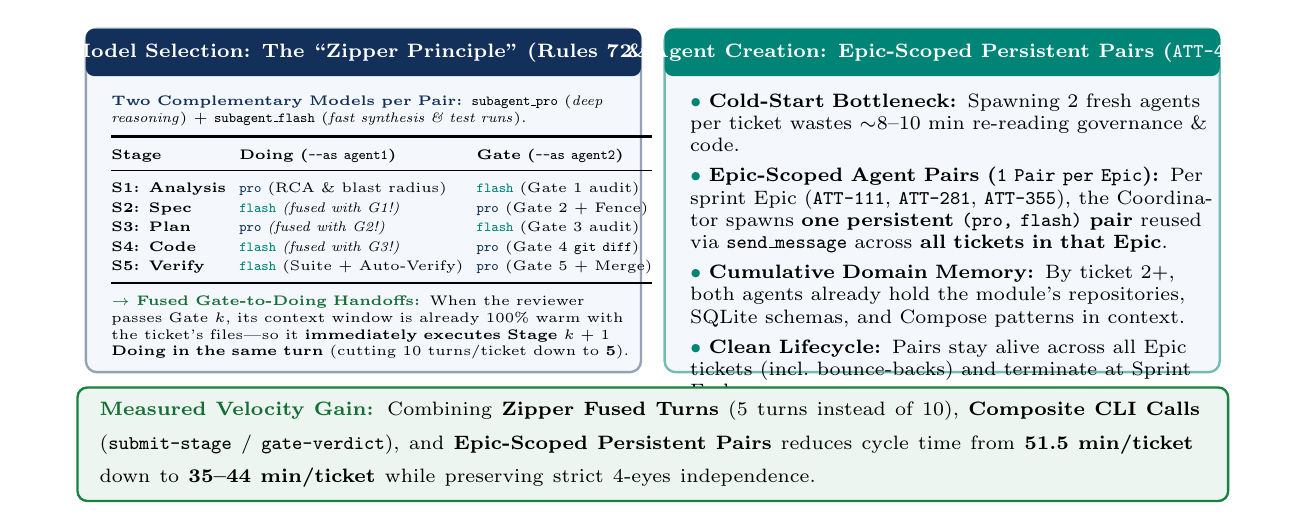
\begin{tikzpicture}[x=1cm, y=1cm]
    % Left Card: The Zipper Principle (Model Selection & Fused Ping-Pong)
    \draw[fill=aaaLightBg, draw=aaaNavy!45, line width=0.85pt, rounded corners=4pt] (-7.20, -1.68) rectangle (-0.15, 2.68);
    \fill[aaaNavy, rounded corners=3pt] (-7.20, 2.08) rectangle (-0.15, 2.68);
    \node[font=\scriptsize\bfseries, text=white] at (-3.675, 2.38)
      {1. Model Selection: The ``Zipper Principle'' (Rules 7 \& 60)};

    \node[anchor=north west, text width=6.65cm, font=\tiny] at (-7.00, 1.96) {
      \textbf{\color{aaaNavy}Two Complementary Models per Pair:}
      \textbf{\texttt{subagent\_pro}} (\emph{deep reasoning}) + \textbf{\texttt{subagent\_flash}} (\emph{fast synthesis \& test runs}).\\[2.5pt]
      {\setlength{\tabcolsep}{2.4pt}
      \renewcommand{\arraystretch}{1.18}
      \begin{tabular}{@{}l l l@{}}
        \toprule
        \textbf{Stage} & \textbf{Doing (\texttt{--as agent1})} & \textbf{Gate (\texttt{--as agent2})} \\
        \midrule
        \textbf{S1: Analysis} & \textcolor{aaaNavy}{\textbf{\texttt{pro}}} (RCA \& blast radius) & \textcolor{aaaTeal}{\textbf{\texttt{flash}}} (Gate 1 audit) \\
        \textbf{S2: Spec} & \textcolor{aaaTeal}{\textbf{\texttt{flash}}} \emph{(fused with G1!)} & \textcolor{aaaNavy}{\textbf{\texttt{pro}}} (Gate 2 + Fence) \\
        \textbf{S3: Plan} & \textcolor{aaaNavy}{\textbf{\texttt{pro}}} \emph{(fused with G2!)} & \textcolor{aaaTeal}{\textbf{\texttt{flash}}} (Gate 3 audit) \\
        \textbf{S4: Code} & \textcolor{aaaTeal}{\textbf{\texttt{flash}}} \emph{(fused with G3!)} & \textcolor{aaaNavy}{\textbf{\texttt{pro}}} (Gate 4 \texttt{git diff}) \\
        \textbf{S5: Verify} & \textcolor{aaaTeal}{\textbf{\texttt{flash}}} (Suite + Auto-Verify) & \textcolor{aaaNavy}{\textbf{\texttt{pro}}} (Gate 5 + Merge) \\
        \bottomrule
      \end{tabular}}\\[3.5pt]
      \textcolor{aaaGreen!85!black}{\textbf{$\rightarrow$ Fused Gate-to-Doing Handoffs:}} When the reviewer passes Gate $k$, its context window is already 100\% warm with the ticket's files—so it \textbf{immediately executes Stage $k+1$ Doing in the same turn} (cutting 10 turns/ticket down to \textbf{5}).
    };

    % Right Card: Epic-Scoped Persistent Agent Pairs
    \draw[fill=aaaLightBg, draw=aaaTeal!55, line width=0.85pt, rounded corners=4pt] (0.15, -1.68) rectangle (7.20, 2.68);
    \fill[aaaTeal, rounded corners=3pt] (0.15, 2.08) rectangle (7.20, 2.68);
    \node[font=\scriptsize\bfseries, text=white] at (3.675, 2.38)
      {2. Agent Creation: Epic-Scoped Persistent Pairs (\texttt{ATT-4520})};

    \node[anchor=north west, text width=6.65cm, font=\scriptsize] at (0.35, 1.98) {
      \bitem \textbf{Cold-Start Bottleneck:} Spawning 2 fresh agents per ticket wastes $\sim$8--10 min re-reading governance \& code.\\[3pt]
      \bitem \textbf{Epic-Scoped Agent Pairs (\texttt{1 Pair per Epic}):}
      Per sprint Epic (\texttt{ATT-111}, \texttt{ATT-281}, \texttt{ATT-355}), the Coordinator spawns \textbf{one persistent \texttt{(pro, flash)} pair} reused via \texttt{send\_message} across \textbf{all tickets in that Epic}.\\[3pt]
      \bitem \textbf{Cumulative Domain Memory:} By ticket 2+, both agents already hold the module's repositories, SQLite schemas, and Compose patterns in context.\\[3pt]
      \bitem \textbf{Clean Lifecycle:} Pairs stay alive across all Epic tickets (incl.\ bounce-backs) and terminate at Sprint End.
    };

    % Bottom Banner
    \node[bannerGreen, text width=14.05cm, anchor=north] at (0, -1.86) {
      \scriptsize\textcolor{aaaGreen!85!black}{\textbf{Measured Velocity Gain:}}
      Combining \textbf{Zipper Fused Turns} (5 turns instead of 10), \textbf{Composite CLI Calls} (\texttt{submit-stage} / \texttt{gate-verdict}), and \textbf{Epic-Scoped Persistent Pairs} reduces cycle time from \textbf{51.5 min/ticket} down to \textbf{35--44 min/ticket} while preserving strict 4-eyes independence.
    };
  \end{tikzpicture}
\end{frame}

% =========================================================================
% SLIDE 8: WORKFLOW 5 — CEREMONY 2 DECISION TREE
% =========================================================================
\begin{frame}{Workflow 5: Ceremony 2 — Joint Review \& Decision Tree}
  \centering
  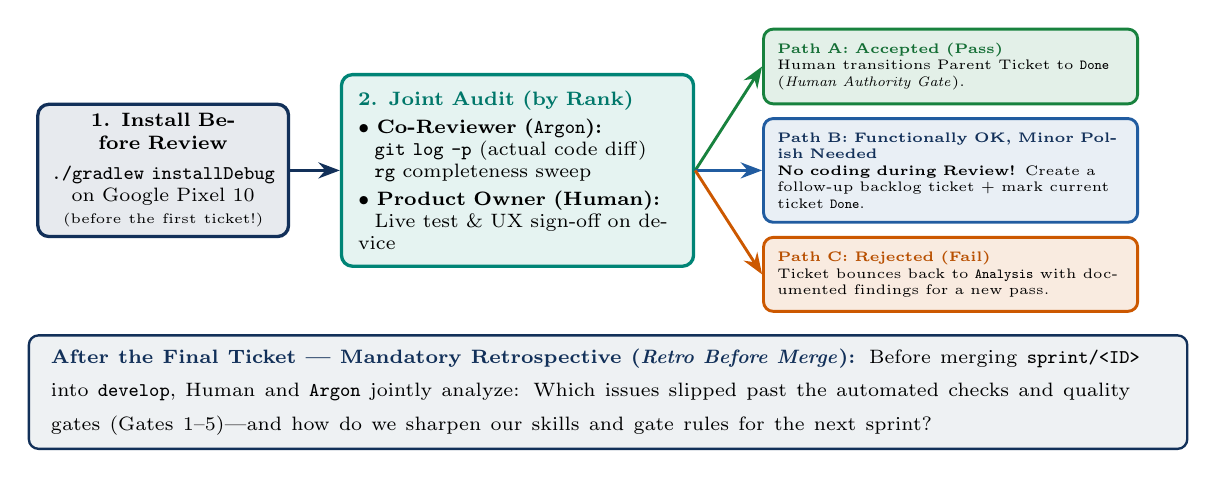
\begin{tikzpicture}[
    x=1cm, y=1cm,
    stepBox/.style={rectangle, rounded corners=4pt, draw=aaaNavy, very thick, fill=aaaNavy!10, text width=2.95cm, align=center, minimum height=1.40cm, font=\scriptsize},
    auditBox/.style={rectangle, rounded corners=4pt, draw=aaaTeal, very thick, fill=aaaTeal!10, text width=4.05cm, align=left, minimum height=2.00cm, inner sep=6pt, font=\scriptsize},
    decBox/.style={rectangle, rounded corners=3.5pt, line width=1.05pt, text width=4.40cm, align=left, minimum height=0.92cm, inner sep=5pt, font=\tiny},
    arr/.style={-{Stealth[scale=1.0]}, line width=1.05pt, draw=aaaNavy}
  ]
    % Step 1: Install on Pixel 10
    \node[stepBox] (inst) at (-5.65, 0.30)
      {\textbf{1. Install Before Review}\\[3pt]\texttt{./gradlew installDebug}\\on Google Pixel 10\\{\tiny(before the first ticket!)}};

    % Step 2: Joint Audit
    \node[auditBox] (aud) at (-1.15, 0.30)
      {\textcolor{aaaTeal!90!black}{\textbf{2. Joint Audit (by Rank)}}\\[2pt]
       $\bullet$ \textbf{Co-Reviewer (\texttt{Argon}):}\\
       \hspace*{6pt}\texttt{git log -p} (actual code diff)\\
       \hspace*{6pt}\texttt{rg} completeness sweep\\[2pt]
       $\bullet$ \textbf{Product Owner (Human):}\\
       \hspace*{6pt}Live test \& UX sign-off on device};

    % Step 3: 3 Decision Paths
    \node[decBox, draw=aaaGreen, fill=aaaGreen!12] (d1) at (4.35, 1.62)
      {\textcolor{aaaGreen!85!black}{\textbf{Path A: Accepted (Pass)}}\\
       Human transitions Parent Ticket to \texttt{Done} (\emph{Human Authority Gate}).};

    \node[decBox, draw=aaaBlue, fill=aaaBlue!10] (d2) at (4.35, 0.30)
      {\textcolor{aaaNavy}{\textbf{Path B: Functionally OK, Minor Polish Needed}}\\
       \textbf{No coding during Review!} Create a follow-up backlog ticket + mark current ticket \texttt{Done}.};

    \node[decBox, draw=aaaAmber, fill=aaaAmber!12] (d3) at (4.35, -1.02)
      {\textcolor{aaaAmber!90!black}{\textbf{Path C: Rejected (Fail)}}\\
       Ticket bounces back to \texttt{Analysis} with documented findings for a new pass.};

    % Connections
    \draw[arr] (inst.east) -- (aud.west);
    \draw[arr, draw=aaaGreen] (aud.east) -- (d1.west);
    \draw[arr, draw=aaaBlue]  (aud.east) -- (d2.west);
    \draw[arr, draw=aaaAmber] (aud.east) -- (d3.west);

    % Bottom Ceremony 2 Golden Rule Banner
    \node[bannerNavy, text width=14.15cm, anchor=north] at (0, -1.78) {
      \scriptsize\textcolor{aaaNavy}{\textbf{After the Final Ticket — Mandatory Retrospective (\emph{Retro Before Merge}):}}
      Before merging \texttt{sprint/<ID>} into \texttt{develop}, Human and \texttt{Argon} jointly analyze: Which issues slipped past the automated checks and quality gates (Gates 1--5)—and how do we sharpen our skills and gate rules for the next sprint?
    };
  \end{tikzpicture}
\end{frame}

% =========================================================================
% SLIDE 9: DETAILED GATE CRITERIA — STAGE 1 & STAGE 2
% =========================================================================
\begin{frame}{Detailed Gate Criteria: Stage 1 (Gate 1) \& Stage 2 (Gate 2)}
  \centering
  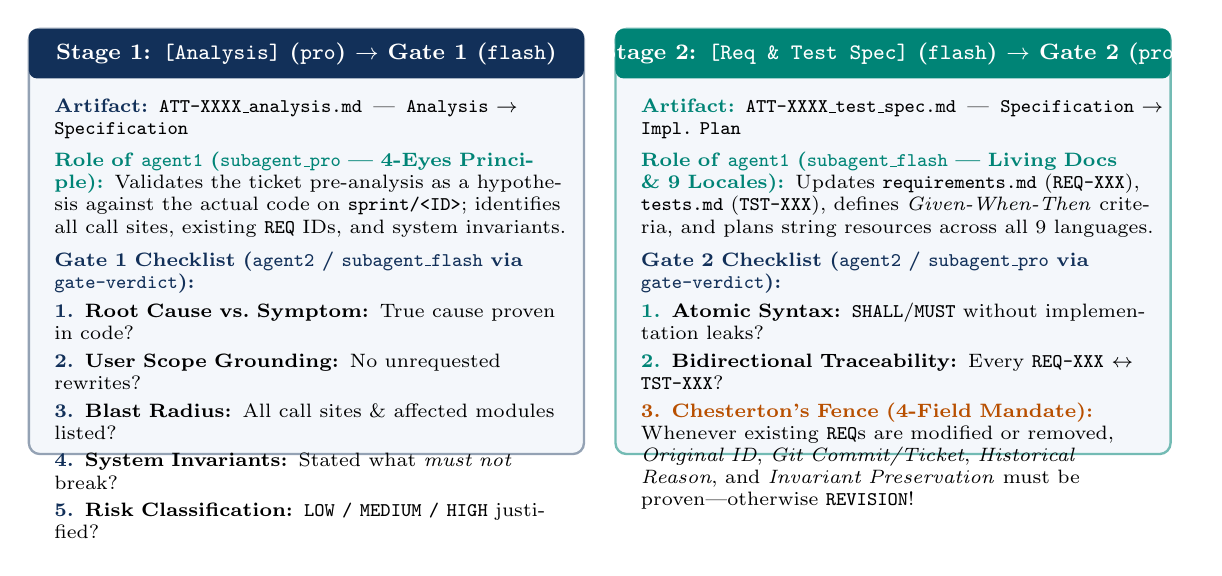
\begin{tikzpicture}[x=1cm, y=1cm]
    % Left Card: Stage 1 -> Gate 1
    \draw[fill=aaaLightBg, draw=aaaNavy!45, line width=0.85pt, rounded corners=4pt] (-7.25, -2.75) rectangle (-0.20, 2.65);
    \fill[aaaNavy, rounded corners=3pt] (-7.25, 2.02) rectangle (-0.20, 2.65);
    \node[font=\footnotesize\bfseries, text=white] at (-3.725, 2.33)
      {Stage 1: \texttt{[Analysis]} (\texttt{pro}) $\rightarrow$ \textbf{Gate 1} (\texttt{flash})};

    \node[anchor=north west, text width=6.65cm, font=\scriptsize] at (-7.05, 1.88) {
      \textbf{\color{aaaNavy}Artifact:} \texttt{ATT-XXXX\_analysis.md} \,|\, \texttt{Analysis} $\rightarrow$ \texttt{Specification}\\[3.5pt]
      \textbf{\color{aaaTeal}Role of \texttt{agent1} (\texttt{subagent\_pro} — 4-Eyes Principle):}
      Validates the ticket pre-analysis as a hypothesis against the actual code on \texttt{sprint/<ID>}; identifies all call sites, existing \texttt{REQ} IDs, and system invariants.\\[4pt]
      \textbf{\color{aaaNavy}Gate 1 Checklist (\texttt{agent2} / \texttt{subagent\_flash} via \texttt{gate-verdict}):}\\[2.5pt]
      \textbf{\color{aaaNavy}1.} \textbf{Root Cause vs.\ Symptom:} True cause proven in code?\\[2pt]
      \textbf{\color{aaaNavy}2.} \textbf{User Scope Grounding:} No unrequested rewrites?\\[2pt]
      \textbf{\color{aaaNavy}3.} \textbf{Blast Radius:} All call sites \& affected modules listed?\\[2pt]
      \textbf{\color{aaaNavy}4.} \textbf{System Invariants:} Stated what \emph{must not} break?\\[2pt]
      \textbf{\color{aaaNavy}5.} \textbf{Risk Classification:} \texttt{LOW / MEDIUM / HIGH} justified?
    };

    % Right Card: Stage 2 -> Gate 2
    \draw[fill=aaaLightBg, draw=aaaTeal!55, line width=0.85pt, rounded corners=4pt] (0.20, -2.75) rectangle (7.25, 2.65);
    \fill[aaaTeal, rounded corners=3pt] (0.20, 2.02) rectangle (7.25, 2.65);
    \node[font=\footnotesize\bfseries, text=white] at (3.725, 2.33)
      {Stage 2: \texttt{[Req \& Test Spec]} (\texttt{flash}) $\rightarrow$ \textbf{Gate 2} (\texttt{pro})};

    \node[anchor=north west, text width=6.65cm, font=\scriptsize] at (0.40, 1.88) {
      \textbf{\color{aaaTeal}Artifact:} \texttt{ATT-XXXX\_test\_spec.md} \,|\, \texttt{Specification} $\rightarrow$ \texttt{Impl.\ Plan}\\[3.5pt]
      \textbf{\color{aaaTeal}Role of \texttt{agent1} (\texttt{subagent\_flash} — Living Docs \& 9 Locales):}
      Updates \texttt{requirements.md} (\texttt{REQ-XXX}), \texttt{tests.md} (\texttt{TST-XXX}), defines \emph{Given-When-Then} criteria, and plans string resources across all 9 languages.\\[4pt]
      \textbf{\color{aaaNavy}Gate 2 Checklist (\texttt{agent2} / \texttt{subagent\_pro} via \texttt{gate-verdict}):}\\[2.5pt]
      \textbf{\color{aaaTeal}1.} \textbf{Atomic Syntax:} \texttt{SHALL}/\texttt{MUST} without implementation leaks?\\[2pt]
      \textbf{\color{aaaTeal}2.} \textbf{Bidirectional Traceability:} Every \texttt{REQ-XXX} $\leftrightarrow$ \texttt{TST-XXX}?\\[2pt]
      \textbf{\color{aaaAmber!90!black}3. Chesterton's Fence (4-Field Mandate):} Whenever existing \texttt{REQ}s are modified or removed, \emph{Original ID}, \emph{Git Commit/Ticket}, \emph{Historical Reason}, and \emph{Invariant Preservation} must be proven—otherwise \texttt{REVISION}!
    };
  \end{tikzpicture}
\end{frame}

% =========================================================================
% SLIDE 10: DETAILED GATE CRITERIA — STAGES 3, 4 & 5
% =========================================================================
\begin{frame}{Detailed Gate Criteria: Stages 3, 4 \& 5 (Gates 3, 4 \& 5)}
  \centering
  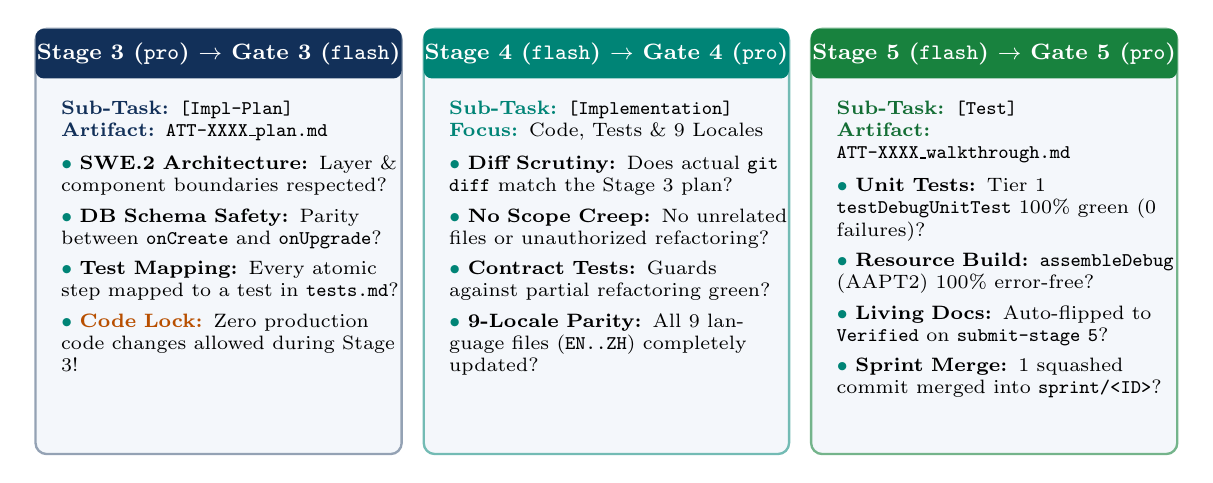
\begin{tikzpicture}[x=1cm, y=1cm]
    % Column 1: Stage 3 -> Gate 3
    \draw[fill=aaaLightBg, draw=aaaNavy!45, line width=0.85pt, rounded corners=4pt] (-7.25, -2.75) rectangle (-2.60, 2.65);
    \fill[aaaNavy, rounded corners=3pt] (-7.25, 2.02) rectangle (-2.60, 2.65);
    \node[font=\footnotesize\bfseries, text=white] at (-4.925, 2.33) {Stage 3 (\texttt{pro}) $\rightarrow$ \textbf{Gate 3} (\texttt{flash})};
    \node[anchor=north west, text width=4.30cm, font=\scriptsize] at (-7.05, 1.86) {
      \textbf{\color{aaaNavy}Sub-Task:} \texttt{[Impl-Plan]}\\
      \textbf{\color{aaaNavy}Artifact:} \texttt{ATT-XXXX\_plan.md}\\[4pt]
      \bitem \textbf{SWE.2 Architecture:} Layer \& component boundaries respected?\\[3pt]
      \bitem \textbf{DB Schema Safety:} Parity between \texttt{onCreate} and \texttt{onUpgrade}?\\[3pt]
      \bitem \textbf{Test Mapping:} Every atomic step mapped to a test in \texttt{tests.md}?\\[3pt]
      \bitem \textbf{\color{aaaAmber!90!black}Code Lock:} Zero production code changes allowed during Stage 3!
    };

    % Column 2: Stage 4 -> Gate 4
    \draw[fill=aaaLightBg, draw=aaaTeal!55, line width=0.85pt, rounded corners=4pt] (-2.32, -2.75) rectangle (2.32, 2.65);
    \fill[aaaTeal, rounded corners=3pt] (-2.32, 2.02) rectangle (2.32, 2.65);
    \node[font=\footnotesize\bfseries, text=white] at (0.0, 2.33) {Stage 4 (\texttt{flash}) $\rightarrow$ \textbf{Gate 4} (\texttt{pro})};
    \node[anchor=north west, text width=4.30cm, font=\scriptsize] at (-2.12, 1.86) {
      \textbf{\color{aaaTeal}Sub-Task:} \texttt{[Implementation]}\\
      \textbf{\color{aaaTeal}Focus:} Code, Tests \& 9 Locales\\[4pt]
      \bitem \textbf{Diff Scrutiny:} Does actual \texttt{git diff} match the Stage 3 plan?\\[3pt]
      \bitem \textbf{No Scope Creep:} No unrelated files or unauthorized refactoring?\\[3pt]
      \bitem \textbf{Contract Tests:} Guards against partial refactoring green?\\[3pt]
      \bitem \textbf{9-Locale Parity:} All 9 language files (\texttt{EN..ZH}) completely updated?
    };

    % Column 3: Stage 5 -> Gate 5
    \draw[fill=aaaLightBg, draw=aaaGreen!60, line width=0.85pt, rounded corners=4pt] (2.60, -2.75) rectangle (7.25, 2.65);
    \fill[aaaGreen, rounded corners=3pt] (2.60, 2.02) rectangle (7.25, 2.65);
    \node[font=\footnotesize\bfseries, text=white] at (4.925, 2.33) {Stage 5 (\texttt{flash}) $\rightarrow$ \textbf{Gate 5} (\texttt{pro})};
    \node[anchor=north west, text width=4.30cm, font=\scriptsize] at (2.80, 1.86) {
      \textbf{\color{aaaGreen!85!black}Sub-Task:} \texttt{[Test]}\\
      \textbf{\color{aaaGreen!85!black}Artifact:} \texttt{ATT-XXXX\_walkthrough.md}\\[4pt]
      \bitem \textbf{Unit Tests:} Tier 1 \texttt{testDebugUnitTest} 100\% green (0 failures)?\\[3pt]
      \bitem \textbf{Resource Build:} \texttt{assembleDebug} (AAPT2) 100\% error-free?\\[3pt]
      \bitem \textbf{Living Docs:} Auto-flipped to \texttt{Verified} on \texttt{submit-stage 5}?\\[3pt]
      \bitem \textbf{Sprint Merge:} 1 squashed commit merged into \texttt{sprint/<ID>}?
    };
  \end{tikzpicture}
\end{frame}

% =========================================================================
% SLIDE 11: INFINITE AGENT CONTEXT & NO FAST-TRACK
% =========================================================================
\begin{frame}{Infinite Agent Context \& Why We Do Not Allow a ``Fast-Track''}
  \centering
  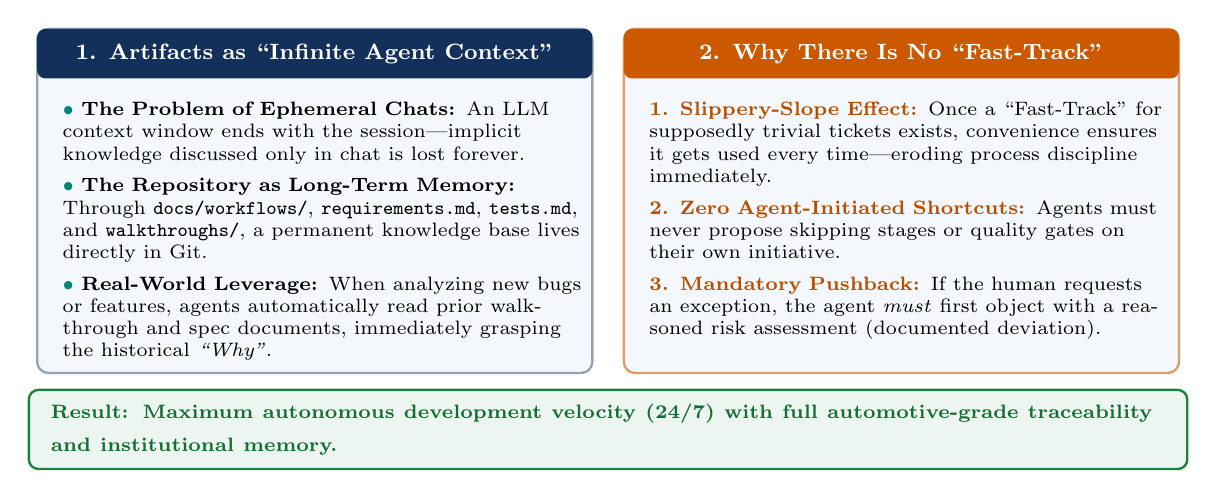
\begin{tikzpicture}[x=1cm, y=1cm]
    % Left Card: Infinite Context
    \draw[fill=aaaLightBg, draw=aaaNavy!45, line width=0.85pt, rounded corners=4pt] (-7.25, -1.72) rectangle (-0.20, 2.65);
    \fill[aaaNavy, rounded corners=3pt] (-7.25, 2.02) rectangle (-0.20, 2.65);
    \node[font=\footnotesize\bfseries, text=white] at (-3.725, 2.33)
      {1. Artifacts as ``Infinite Agent Context''};

    \node[anchor=north west, text width=6.65cm, font=\scriptsize] at (-7.05, 1.84) {
      \bitem \textbf{The Problem of Ephemeral Chats:} An LLM context window ends with the session—implicit knowledge discussed only in chat is lost forever.\\[3.5pt]
      \bitem \textbf{The Repository as Long-Term Memory:} Through \texttt{docs/workflows/}, \texttt{requirements.md}, \texttt{tests.md}, and \texttt{walkthroughs/}, a permanent knowledge base lives directly in Git.\\[3.5pt]
      \bitem \textbf{Real-World Leverage:} When analyzing new bugs or features, agents automatically read prior walkthrough and spec documents, immediately grasping the historical \emph{``Why''}.
    };

    % Right Card: No Fast-Track / Exceptions only under protest
    \draw[fill=aaaLightBg, draw=aaaAmber!60, line width=0.85pt, rounded corners=4pt] (0.20, -1.72) rectangle (7.25, 2.65);
    \fill[aaaAmber, rounded corners=3pt] (0.20, 2.02) rectangle (7.25, 2.65);
    \node[font=\footnotesize\bfseries, text=white] at (3.725, 2.33)
      {2. Why There Is No ``Fast-Track''};

    \node[anchor=north west, text width=6.65cm, font=\scriptsize] at (0.40, 1.84) {
      \textbf{\color{aaaAmber!90!black}1. Slippery-Slope Effect:} Once a ``Fast-Track'' for supposedly trivial tickets exists, convenience ensures it gets used every time—eroding process discipline immediately.\\[3.5pt]
      \textbf{\color{aaaAmber!90!black}2. Zero Agent-Initiated Shortcuts:} Agents must never propose skipping stages or quality gates on their own initiative.\\[3.5pt]
      \textbf{\color{aaaAmber!90!black}3. Mandatory Pushback:} If the human requests an exception, the agent \emph{must} first object with a reasoned risk assessment (documented deviation).
    };

    % Bottom Conclusion Banner
    \node[bannerGreen, text width=14.15cm, anchor=north] at (0, -1.92) {
      \centering\scriptsize\textcolor{aaaGreen!85!black}{\textbf{Result: Maximum autonomous development velocity (24/7) with full automotive-grade traceability and institutional memory.}}
    };
  \end{tikzpicture}
\end{frame}

% =========================================================================
% SLIDE 12: CASCADE CONTROL (CONTROL ENGINEERING PRINCIPLE)
% =========================================================================
\begin{frame}{Control Engineering Principle: Agile Agentic ASPICE as Cascade Control}
  \centering
  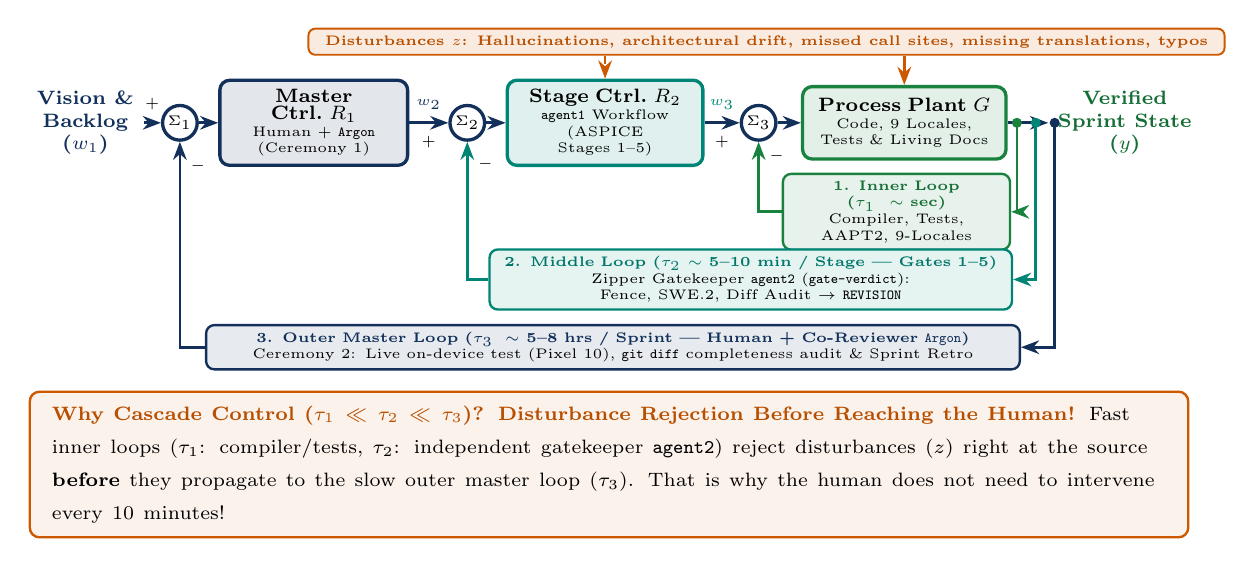
\begin{tikzpicture}[
    x=1cm, y=1cm,
    sum/.style={circle, draw=aaaNavy, very thick, fill=white, minimum size=0.44cm, inner sep=0pt, font=\tiny\bfseries},
    reg1/.style={rectangle, rounded corners=3.5pt, draw=aaaNavy, very thick, fill=aaaNavy!12, text width=2.15cm, align=center, minimum height=0.92cm, font=\tiny},
    reg2/.style={rectangle, rounded corners=3.5pt, draw=aaaTeal, very thick, fill=aaaTeal!12, text width=2.25cm, align=center, minimum height=0.92cm, font=\tiny},
    plant/.style={rectangle, rounded corners=3.5pt, draw=aaaGreen, very thick, fill=aaaGreen!12, text width=2.35cm, align=center, minimum height=0.92cm, font=\tiny},
    fbBox/.style={rectangle, rounded corners=3pt, line width=0.85pt, align=center, minimum height=0.54cm, inner ysep=2.5pt, font=\tiny},
    sigArr/.style={-{Stealth[scale=0.9]}, line width=0.95pt, draw=aaaNavy},
    distArr/.style={-{Stealth[scale=0.9]}, line width=0.95pt, draw=aaaAmber}
  ]
    % =================== FORWARD PATH (y = 1.65) ===================
    \node[font=\scriptsize\bfseries, text=aaaNavy, align=center] (w1) at (-6.65, 1.65)
      {Vision \&\\Backlog\\($w_1$)};
    \node[sum] (s1) at (-5.45, 1.65) {$\Sigma_1$};
    \node[reg1] (r1) at (-3.75, 1.65)
      {\textbf{\scriptsize Master Ctrl.\ $R_1$}\\Human + \texttt{Argon}\\(Ceremony 1)};
    \node[sum] (s2) at (-1.80, 1.65) {$\Sigma_2$};
    \node[reg2] (r2) at (-0.05, 1.65)
      {\textbf{\scriptsize Stage Ctrl.\ $R_2$}\\\texttt{agent1} Workflow\\(ASPICE Stages 1--5)};
    \node[sum] (s3) at (1.90, 1.65) {$\Sigma_3$};
    \node[plant] (g) at (3.75, 1.65)
      {\textbf{\scriptsize Process Plant $G$}\\Code, 9 Locales,\\Tests \& Living Docs};
    \node[font=\scriptsize\bfseries, text=aaaGreen!85!black, align=center] (y) at (6.55, 1.65)
      {Verified\\Sprint State\\($y$)};

    % Forward Connections with Setpoint Labels (w1 -> w2 -> w3 -> y)
    \draw[sigArr] (w1) -- node[above=1pt, font=\tiny\bfseries] {$+$} (s1);
    \draw[sigArr] (s1) -- (r1);
    \draw[sigArr] (r1) -- node[above=1pt, font=\tiny\bfseries, text=aaaNavy] {$w_2$} node[below=1pt, font=\tiny] {$+$} (s2);
    \draw[sigArr] (s2) -- (r2);
    \draw[sigArr] (r2) -- node[above=1pt, font=\tiny\bfseries, text=aaaTeal] {$w_3$} node[below=1pt, font=\tiny] {$+$} (s3);
    \draw[sigArr] (s3) -- (g);
    \draw[sigArr] (g) -- (y);

    % Tap points on output line
    \filldraw[aaaGreen] (5.18, 1.65) circle (1.6pt);
    \filldraw[aaaTeal]  (5.42, 1.65) circle (1.6pt);
    \filldraw[aaaNavy]  (5.66, 1.65) circle (1.6pt);

    % =================== DISTURBANCES z (y = 2.68) ===================
    \node[rectangle, rounded corners=2.5pt, fill=aaaAmber!12, draw=aaaAmber, line width=0.7pt,
          font=\tiny\bfseries, text=aaaAmber!90!black, inner xsep=6pt, inner ysep=2.5pt] (z) at (2.00, 2.68)
      {Disturbances $z$: Hallucinations, architectural drift, missed call sites, missing translations, typos};
    \draw[distArr] (z.south -| g.north) -- (g.north);
    \draw[distArr, dashed] (z.south -| r2.north) -- (r2.north);

    % =================== LOOP 1: INNERMOST FAST LOOP (y = 0.52, strictly 2 lines) ===================
    \node[fbBox, draw=aaaGreen, fill=aaaGreen!10, text width=2.65cm] (fb3) at (3.65, 0.52)
      {\textcolor{aaaGreen!85!black}{\textbf{1. Inner Loop ($\tau_1 \sim$ sec)}}\\Compiler, Tests, AAPT2, 9-Locales};
    \draw[sigArr, draw=aaaGreen] (5.18, 1.65) |- (fb3.east);
    \draw[sigArr, draw=aaaGreen] (fb3.west) -| node[pos=0.90, right, font=\tiny\bfseries] {$-$} (s3.south);

    % =================== LOOP 2: MIDDLE ASPICE GATE LOOP (y = -0.34, strictly 2 lines) ===================
    \node[fbBox, draw=aaaTeal, fill=aaaTeal!10, text width=6.40cm] (fb2) at (1.80, -0.34)
      {\textcolor{aaaTeal!90!black}{\textbf{2. Middle Loop ($\tau_2 \sim$ 5--10 min / Stage — Gates 1--5)}}\\Zipper Gatekeeper \texttt{agent2} (\texttt{gate-verdict}): Fence, SWE.2, Diff Audit $\rightarrow$ \texttt{REVISION}};
    \draw[sigArr, draw=aaaTeal] (5.42, 1.65) |- (fb2.east);
    \draw[sigArr, draw=aaaTeal] (fb2.west) -| node[pos=0.92, right, font=\tiny\bfseries] {$-$} (s2.south);

    % =================== LOOP 3: OUTER HUMAN LOOP (y = -1.20, strictly 2 lines) ===================
    \node[fbBox, draw=aaaNavy, fill=aaaNavy!10, text width=10.10cm] (fb1) at (0.05, -1.20)
      {\textcolor{aaaNavy}{\textbf{3. Outer Master Loop ($\tau_3 \sim$ 5--8 hrs / Sprint — Human + Co-Reviewer \texttt{Argon})}}\\Ceremony 2: Live on-device test (Pixel 10), \texttt{git diff} completeness audit \& Sprint Retro};
    \draw[sigArr, draw=aaaNavy] (5.66, 1.65) |- (fb1.east);
    \draw[sigArr, draw=aaaNavy] (fb1.west) -| node[pos=0.94, right, font=\tiny\bfseries] {$-$} (s1.south);

    % Bottom Takeaway Banner
    \node[bannerAmber, text width=14.15cm, anchor=north] at (0, -1.75) {
      \scriptsize\textcolor{aaaAmber!90!black}{\textbf{Why Cascade Control ($\tau_1 \ll \tau_2 \ll \tau_3$)? Disturbance Rejection Before Reaching the Human!}}
      Fast inner loops ($\tau_1$: compiler/tests, $\tau_2$: independent gatekeeper \texttt{agent2}) reject disturbances ($z$) right at the source \textbf{before} they propagate to the slow outer master loop ($\tau_3$). That is why the human does not need to intervene every 10 minutes!
    };
  \end{tikzpicture}
\end{frame}

% =========================================================================
% SLIDE 12 (FORMERLY SLIDE 3): TIME ALLOCATION (VIBE CODING VS. AAA)
% =========================================================================
\begin{frame}{Time Allocation: Vibe Coding vs.\ Agile Agentic ASPICE}
  \centering
  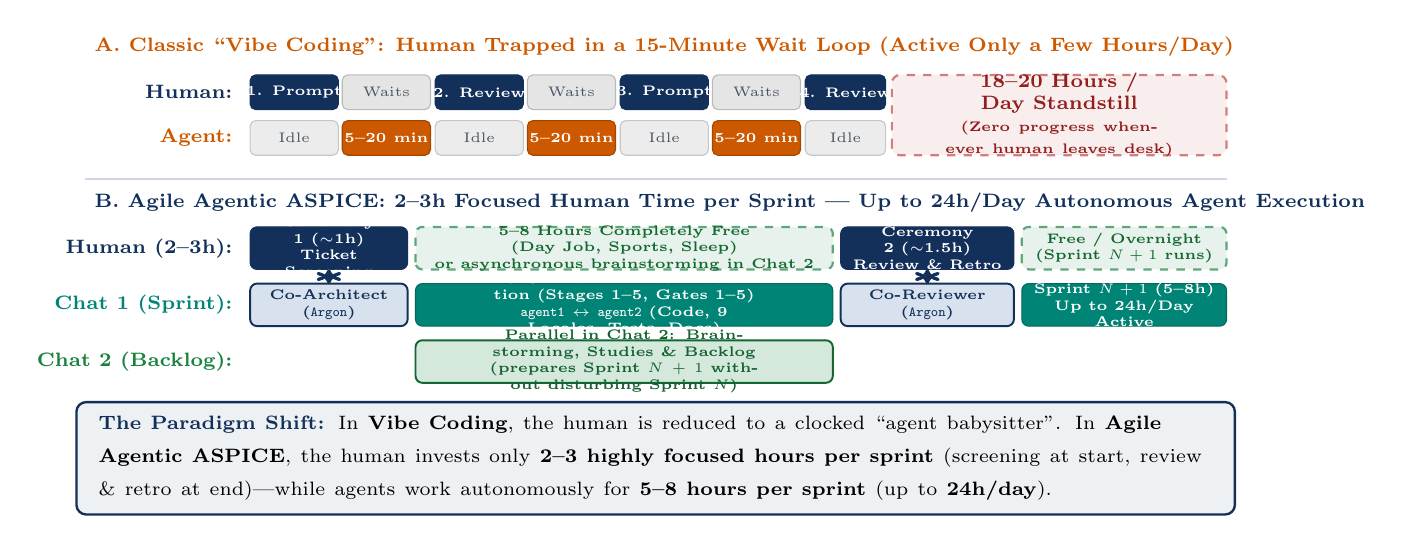
\begin{tikzpicture}[x=1cm, y=1cm]
    % ----------------------- PART A: VIBE CODING -----------------------
    \node[anchor=west, font=\scriptsize\bfseries, text=aaaAmber] at (-7.25, 2.78)
      {A. Classic ``Vibe Coding'': Human Trapped in a 15-Minute Wait Loop (Active Only a Few Hours/Day)};

    % Row labels
    \node[anchor=east, font=\scriptsize\bfseries, text=aaaNavy] at (-5.25, 2.20) {Human:};
    \node[anchor=east, font=\scriptsize\bfseries, text=aaaAmber] at (-5.25, 1.62) {Agent:};

    % 3 repeating Vibe cycles (each 2.30cm wide: 1.12cm Human + 1.12cm Agent)
    \foreach \x/\lblA in {-5.15/1. Prompt, -2.80/2. Review, -0.45/3. Prompt} {
      % Human gives prompt / checks
      \draw[fill=aaaNavy, draw=aaaNavy, rounded corners=2pt] (\x, 1.98) rectangle (\x+1.12, 2.42);
      \node[font=\tiny\bfseries, text=white] at (\x+0.56, 2.20) {\lblA};
      % Agent Idle
      \draw[fill=gray!15, draw=gray!45, rounded corners=2pt] (\x, 1.40) rectangle (\x+1.12, 1.84);
      \node[font=\tiny, text=aaaSlate] at (\x+0.56, 1.62) {Idle};

      % Human waits while Agent works 5-20m
      \draw[fill=gray!20, draw=gray!55, rounded corners=2pt] (\x+1.17, 1.98) rectangle (\x+2.29, 2.42);
      \node[font=\tiny, text=aaaSlate] at (\x+1.73, 2.20) {Waits};
      % Agent works
      \draw[fill=aaaAmber, draw=aaaAmber!80!black, rounded corners=2pt] (\x+1.17, 1.40) rectangle (\x+2.29, 1.84);
      \node[font=\tiny\bfseries, text=white] at (\x+1.73, 1.62) {5--20 min};
    }

    % Final check before stopping
    \draw[fill=aaaNavy, draw=aaaNavy, rounded corners=2pt] (1.90, 1.98) rectangle (2.92, 2.42);
    \node[font=\tiny\bfseries, text=white] at (2.41, 2.20) {4. Review};
    \draw[fill=gray!15, draw=gray!45, rounded corners=2pt] (1.90, 1.40) rectangle (2.92, 1.84);
    \node[font=\tiny, text=aaaSlate] at (2.41, 1.62) {Idle};

    % 18-20h Standstill block
    \draw[fill=aaaRed!8, draw=aaaRed!60, dashed, line width=0.8pt, rounded corners=3pt] (3.00, 1.40) rectangle (7.25, 2.42);
    \node[font=\scriptsize\bfseries, text=aaaRed!80!black, align=center, text width=4.05cm] at (5.125, 1.91)
      {18--20 Hours / Day Standstill\\{\tiny(Zero progress whenever human leaves desk)}};

    % Divider line
    \draw[line width=0.7pt, draw=aaaBorder] (-7.25, 1.10) -- (7.25, 1.10);

    % ------------------ PART B: AGILE AGENTIC ASPICE ------------------
    \node[anchor=west, font=\scriptsize\bfseries, text=aaaNavy] at (-7.25, 0.80)
      {B. Agile Agentic ASPICE: 2--3h Focused Human Time per Sprint — Up to 24h/Day Autonomous Agent Execution};

    % Row labels
    \node[anchor=east, font=\scriptsize\bfseries, text=aaaNavy] at (-5.25, 0.22) {Human (2--3h):};
    \node[anchor=east, font=\scriptsize\bfseries, text=aaaTeal] at (-5.25, -0.50) {Chat 1 (Sprint):};
    \node[anchor=east, font=\scriptsize\bfseries, text=aaaGreen] at (-5.25, -1.22) {Chat 2 (Backlog):};

    % --- Row 1: Human ---
    \draw[fill=aaaNavy, draw=aaaNavy, rounded corners=2.5pt] (-5.15, -0.05) rectangle (-3.15, 0.49);
    \node[font=\tiny\bfseries, text=white, align=center, text width=1.9cm] at (-4.15, 0.22)
      {Ceremony 1 ($\sim$1h)\\Ticket Screening};

    \draw[fill=aaaGreen!10, draw=aaaGreen!70, dashed, line width=0.8pt, rounded corners=2.5pt] (-3.05, -0.05) rectangle (2.25, 0.49);
    \node[font=\tiny\bfseries, text=aaaGreen!80!black, align=center, text width=5.1cm] at (-0.40, 0.22)
      {5--8 Hours Completely Free (Day Job, Sports, Sleep)\\or asynchronous brainstorming in Chat 2};

    \draw[fill=aaaNavy, draw=aaaNavy, rounded corners=2.5pt] (2.35, -0.05) rectangle (4.55, 0.49);
    \node[font=\tiny\bfseries, text=white, align=center, text width=2.1cm] at (3.45, 0.22)
      {Ceremony 2 ($\sim$1.5h)\\Review \& Retro};

    \draw[fill=aaaGreen!10, draw=aaaGreen!70, dashed, line width=0.8pt, rounded corners=2.5pt] (4.65, -0.05) rectangle (7.25, 0.49);
    \node[font=\tiny\bfseries, text=aaaGreen!80!black, align=center, text width=2.4cm] at (5.95, 0.22)
      {Free / Overnight\\(Sprint $N+1$ runs)};

    % --- Row 2: Chat 1 (Sprint Execution Agents) ---
    \draw[fill=aaaBlue!18, draw=aaaNavy, line width=0.7pt, rounded corners=2.5pt] (-5.15, -0.77) rectangle (-3.15, -0.23);
    \node[font=\tiny\bfseries, text=aaaNavy, align=center, text width=1.9cm] at (-4.15, -0.50)
      {Co-Architect\\(\texttt{Argon})};

    \draw[fill=aaaTeal, draw=aaaTeal!80!black, rounded corners=2.5pt] (-3.05, -0.77) rectangle (2.25, -0.23);
    \node[font=\tiny\bfseries, text=white, align=center, text width=5.1cm] at (-0.40, -0.50)
      {5--8h Autonomous Execution (Stages 1--5, Gates 1--5)\\\texttt{agent1} $\leftrightarrow$ \texttt{agent2} (Code, 9 Locales, Tests, Docs)};

    \draw[fill=aaaBlue!18, draw=aaaNavy, line width=0.7pt, rounded corners=2.5pt] (2.35, -0.77) rectangle (4.55, -0.23);
    \node[font=\tiny\bfseries, text=aaaNavy, align=center, text width=2.1cm] at (3.45, -0.50)
      {Co-Reviewer\\(\texttt{Argon})};

    \draw[fill=aaaTeal, draw=aaaTeal!80!black, rounded corners=2.5pt] (4.65, -0.77) rectangle (7.25, -0.23);
    \node[font=\tiny\bfseries, text=white, align=center, text width=2.4cm] at (5.95, -0.50)
      {Sprint $N+1$ (5--8h)\\Up to 24h/Day Active};

    % --- Row 3: Chat 2 (Parallel Brainstorming) ---
    \draw[fill=aaaGreen!18, draw=aaaGreen!80!black, line width=0.7pt, rounded corners=2.5pt] (-3.05, -1.49) rectangle (2.25, -0.95);
    \node[font=\tiny\bfseries, text=aaaGreen!75!black, align=center, text width=5.1cm] at (-0.40, -1.22)
      {Parallel in Chat 2: Brainstorming, Studies \& Backlog\\(prepares Sprint $N+1$ without disturbing Sprint $N$)};

    % Sync arrows between Human and Chat 1
    \draw[<->, very thick, draw=aaaNavy] (-4.15, -0.05) -- (-4.15, -0.23);
    \draw[<->, very thick, draw=aaaNavy] (3.45, -0.05) -- (3.45, -0.23);

    % Bottom Summary Banner
    \node[bannerNavy, text width=14.15cm, anchor=north] at (0, -1.72) {
      \scriptsize\textcolor{aaaNavy}{\textbf{The Paradigm Shift:}}
      In \textbf{Vibe Coding}, the human is reduced to a clocked ``agent babysitter''. In \textbf{Agile Agentic ASPICE}, the human invests only \textbf{2--3 highly focused hours per sprint} (screening at start, review \& retro at end)—while agents work autonomously for \textbf{5--8 hours per sprint} (up to \textbf{24h/day}).
    };
  \end{tikzpicture}
\end{frame}

% =========================================================================
% SLIDE 14: THE LIVING DOCUMENT TRIAD — GOVERNANCE, CODING & DESIGN RULES
% =========================================================================
\begin{frame}{The Living Document Triad: Governance, Coding \& Design Rules}
  \centering
  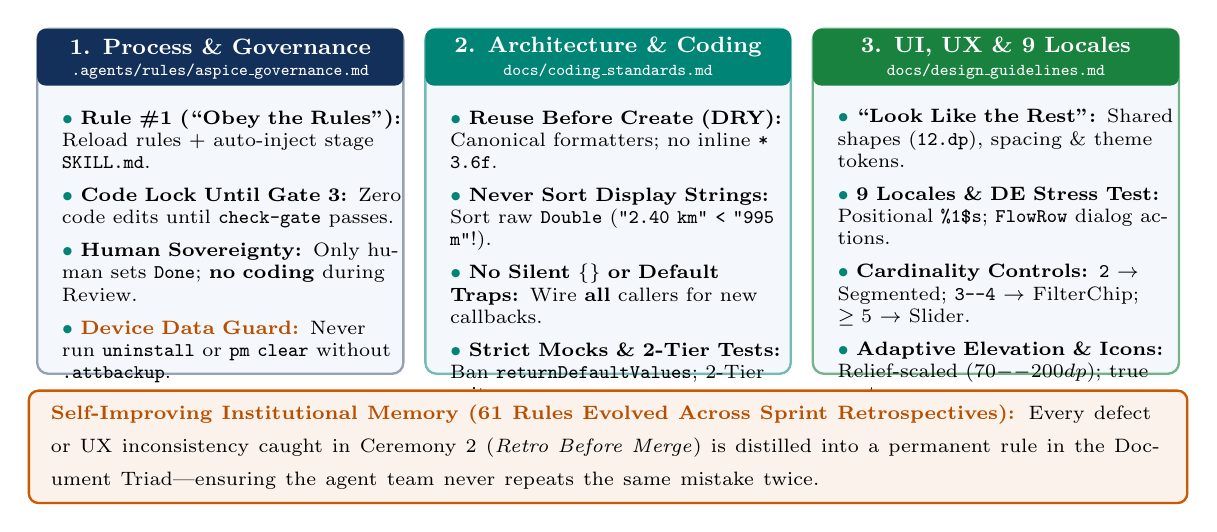
\begin{tikzpicture}[x=1cm, y=1cm]
    % Column 1: Process & Governance Rules
    \draw[fill=aaaLightBg, draw=aaaNavy!45, line width=0.85pt, rounded corners=4pt] (-7.25, -1.68) rectangle (-2.60, 2.70);
    \fill[aaaNavy, rounded corners=3pt] (-7.25, 1.98) rectangle (-2.60, 2.70);
    \node[font=\footnotesize\bfseries, text=white] at (-4.925, 2.47) {1. Process \& Governance};
    \node[font=\fontsize{6}{7}\selectfont\ttfamily, text=white!90] at (-4.925, 2.16) {.agents/rules/aspice\_governance.md};
    \node[anchor=north west, text width=4.32cm, font=\scriptsize] at (-7.06, 1.80) {
      \bitem \textbf{Rule \#1 (``Obey the Rules''):} Reload rules + auto-inject stage \texttt{SKILL.md}.\\[4pt]
      \bitem \textbf{Code Lock Until Gate 3:} Zero code edits until \texttt{check-gate} passes.\\[4pt]
      \bitem \textbf{Human Sovereignty:} Only human sets \texttt{Done}; \textbf{no coding} during Review.\\[4pt]
      \bitem \textbf{\color{aaaAmber!90!black}Device Data Guard:} Never run \texttt{uninstall} or \texttt{pm clear} without \texttt{.attbackup}.
    };

    % Column 2: Technical Architecture & Coding Standards
    \draw[fill=aaaLightBg, draw=aaaTeal!55, line width=0.85pt, rounded corners=4pt] (-2.32, -1.68) rectangle (2.32, 2.70);
    \fill[aaaTeal, rounded corners=3pt] (-2.32, 1.98) rectangle (2.32, 2.70);
    \node[font=\footnotesize\bfseries, text=white] at (0.0, 2.47) {2. Architecture \& Coding};
    \node[font=\fontsize{6}{7}\selectfont\ttfamily, text=white!90] at (0.0, 2.16) {docs/coding\_standards.md};
    \node[anchor=north west, text width=4.32cm, font=\scriptsize] at (-2.13, 1.80) {
      \bitem \textbf{Reuse Before Create (DRY):} Canonical formatters; no inline \texttt{* 3.6f}.\\[4pt]
      \bitem \textbf{Never Sort Display Strings:} Sort raw \texttt{Double} (\texttt{"2.40 km" < "995 m"}!).\\[4pt]
      \bitem \textbf{No Silent \texttt{\{\}} or Default Traps:} Wire \textbf{all} callers for new callbacks.\\[4pt]
      \bitem \textbf{Strict Mocks \& 2-Tier Tests:} Ban \texttt{returnDefaultValues}; 2-Tier suite.
    };

    % Column 3: UI, UX & 9-Language Design Guidelines
    \draw[fill=aaaLightBg, draw=aaaGreen!60, line width=0.85pt, rounded corners=4pt] (2.60, -1.68) rectangle (7.25, 2.70);
    \fill[aaaGreen, rounded corners=3pt] (2.60, 1.98) rectangle (7.25, 2.70);
    \node[font=\footnotesize\bfseries, text=white] at (4.925, 2.47) {3. UI, UX \& 9 Locales};
    \node[font=\fontsize{6}{7}\selectfont\ttfamily, text=white!90] at (4.925, 2.16) {docs/design\_guidelines.md};
    \node[anchor=north west, text width=4.32cm, font=\scriptsize] at (2.79, 1.80) {
      \bitem \textbf{``Look Like the Rest'':} Shared shapes (\texttt{12.dp}), spacing \& theme tokens.\\[4pt]
      \bitem \textbf{9 Locales \& DE Stress Test:} Positional \texttt{\%1\$s}; \texttt{FlowRow} dialog actions.\\[4pt]
      \bitem \textbf{Cardinality Controls:} \texttt{2} $\rightarrow$ Segmented; \texttt{3--4} $\rightarrow$ FilterChip; $\ge 5$ $\rightarrow$ Slider.\\[4pt]
      \bitem \textbf{Adaptive Elevation \& Icons:} Relief-scaled ($70\text{--}200\text{ dp}$); true vectors.
    };

    % Bottom Self-Improving Memory Banner
    \node[bannerAmber, text width=14.15cm, anchor=north] at (0, -1.88) {
      \scriptsize\textcolor{aaaAmber!90!black}{\textbf{Self-Improving Institutional Memory (61 Rules Evolved Across Sprint Retrospectives):}}
      Every defect or UX inconsistency caught in Ceremony 2 (\emph{Retro Before Merge}) is distilled into a permanent rule in the Document Triad—ensuring the agent team never repeats the same mistake twice.
    };
  \end{tikzpicture}
\end{frame}

% =========================================================================
% SLIDE 15: EMPIRICAL EVOLUTION OF FORMAL REQUIREMENTS (REQ-*)
% =========================================================================
\begin{frame}{Empirical Impact: Evolution of Formal Requirements (\texttt{REQ-*})}
  \centering
  \resizebox{!}{0.82\textheight}{%
  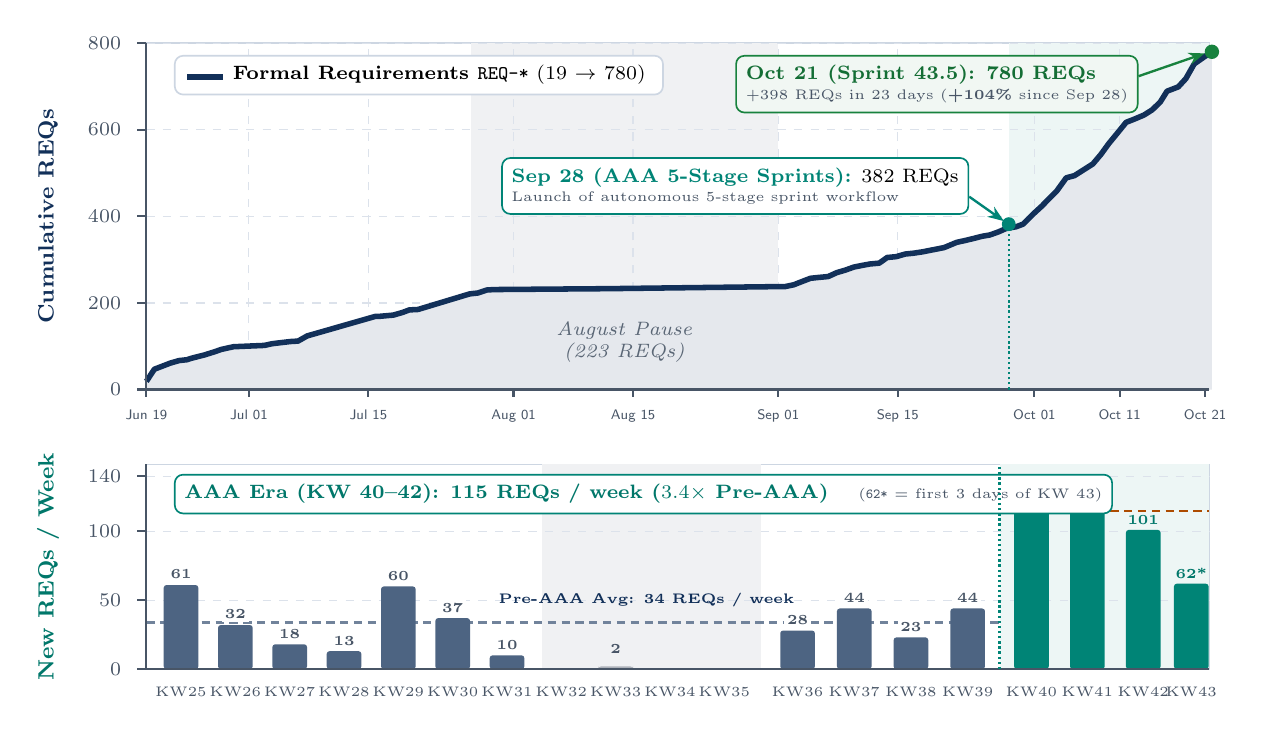
\begin{tikzpicture}[
    x=1cm, y=1cm,
    gridLine/.style={draw=aaaBorder!70, dashed, line width=0.45pt},
    axisLine/.style={draw=aaaSlate, line width=0.8pt},
    milestone/.style={draw=aaaAmber!80, densely dotted, line width=0.85pt},
    callout/.style={rectangle, rounded corners=3pt, fill=white, draw=aaaBorder, line width=0.6pt, inner sep=3.5pt, font=\scriptsize, align=left}
  ]
    % Panel backgrounds
    \fill[white, draw=aaaBorder, line width=0.6pt] (0, 0) rectangle (13.5, 4.4);
    \fill[white, draw=aaaBorder, line width=0.6pt] (0, -3.55) rectangle (13.5, -0.95);

    % Summer break shaded band (Jul 27 - Sep 01)
    \fill[aaaSlate!8] (4.12, 0) rectangle (8.024, 4.4);
    \fill[aaaSlate!8] (5.03, -3.55) rectangle (7.80, -0.95);

    % AAA Era shaded band (Sep 28 - Oct 21)
    \fill[aaaTeal!7] (10.952, 0) rectangle (13.5, 4.4);
    \fill[aaaTeal!7] (10.835, -3.55) rectangle (13.5, -0.95);

    % Top Panel Grid & Ticks (y scaled by 4.4/4.8 = 0.9167)
    \foreach \x/\lbl in {0.0/Jun 19, 1.301/Jul 01, 2.819/Jul 15, 4.663/Aug 01, 6.181/Aug 15, 8.024/Sep 01, 9.542/Sep 15, 11.277/Oct 01, 12.361/Oct 11, 13.446/Oct 21} {
      \draw[gridLine] (\x, 0) -- (\x, 4.4);
      \draw[axisLine] (\x, 0) -- (\x, -0.09) node[below=1pt, font=\tiny\sffamily\mdseries, text=aaaSlate] {\lbl};
    }

    \foreach \r/\yl in {0/0.0, 200/1.1, 400/2.2, 600/3.3, 800/4.4} {
      \draw[gridLine] (0, \yl) -- (13.5, \yl);
      \draw[axisLine] (0, \yl) -- (-0.12, \yl) node[left=2pt, font=\scriptsize\mdseries, text=aaaSlate] {\r};
    }

    % Bottom Panel Horizontal Grid (0, 50, 100, 140 REQs/week)
    \foreach \w/\yl in {0/-3.55, 50/-2.675, 100/-1.80, 140/-1.10} {
      \draw[gridLine] (0, \yl) -- (13.5, \yl);
      \draw[axisLine] (0, \yl) -- (-0.12, \yl) node[left=2pt, font=\scriptsize\mdseries, text=aaaSlate] {\w};
    }

    % Top Panel Shaded Area & REQ-* Curve
    \begin{scope}[yscale=0.9167]
      \fill[aaaNavy!11] (0,0) -- (0.0,0.114) -- (0.101,0.282) -- (0.301,0.366) -- (0.414,0.402) -- (0.517,0.414) -- (0.564,0.432) -- (0.737,0.48) -- (0.86,0.522) -- (0.956,0.558) -- (1.107,0.594) -- (1.498,0.612) -- (1.598,0.636) -- (1.83,0.666) -- (1.926,0.672) -- (2.043,0.744) -- (2.907,1.014) -- (2.951,1.014) -- (3.136,1.032) -- (3.251,1.068) -- (3.339,1.104) -- (3.45,1.11) -- (4.106,1.326) -- (4.208,1.338) -- (4.325,1.38) -- (4.42,1.386) -- (5.838,1.398) -- (8.115,1.428) -- (8.221,1.452) -- (8.333,1.5) -- (8.434,1.542) -- (8.538,1.554) -- (8.658,1.566) -- (8.767,1.62) -- (8.878,1.656) -- (8.986,1.698) -- (9.097,1.722) -- (9.188,1.74) -- (9.307,1.752) -- (9.408,1.83) -- (9.523,1.842) -- (9.637,1.878) -- (9.745,1.89) -- (9.854,1.908) -- (9.966,1.932) -- (10.079,1.956) -- (10.132,1.968) -- (10.291,2.04) -- (10.392,2.064) -- (10.506,2.094) -- (10.614,2.124) -- (10.711,2.142) -- (10.819,2.184) -- (10.919,2.232) -- (11.046,2.256) -- (11.133,2.292) -- (11.266,2.436) -- (11.374,2.544) -- (11.464,2.646) -- (11.559,2.748) -- (11.682,2.934) -- (11.786,2.964) -- (12.02,3.126) -- (12.122,3.258) -- (12.222,3.408) -- (12.335,3.558) -- (12.442,3.702) -- (12.553,3.75) -- (12.67,3.804) -- (12.774,3.876) -- (12.876,3.984) -- (12.962,4.134) -- (13.105,4.194) -- (13.201,4.308) -- (13.307,4.512) -- (13.425,4.602) -- (13.532,4.68) -- (13.532, 0) -- cycle;
      \draw[draw=aaaNavy, line width=2.0pt, line join=round] (0.0,0.114) -- (0.101,0.282) -- (0.301,0.366) -- (0.414,0.402) -- (0.517,0.414) -- (0.564,0.432) -- (0.737,0.48) -- (0.86,0.522) -- (0.956,0.558) -- (1.107,0.594) -- (1.498,0.612) -- (1.598,0.636) -- (1.83,0.666) -- (1.926,0.672) -- (2.043,0.744) -- (2.907,1.014) -- (2.951,1.014) -- (3.136,1.032) -- (3.251,1.068) -- (3.339,1.104) -- (3.45,1.11) -- (4.106,1.326) -- (4.208,1.338) -- (4.325,1.38) -- (4.42,1.386) -- (5.838,1.398) -- (8.115,1.428) -- (8.221,1.452) -- (8.333,1.5) -- (8.434,1.542) -- (8.538,1.554) -- (8.658,1.566) -- (8.767,1.62) -- (8.878,1.656) -- (8.986,1.698) -- (9.097,1.722) -- (9.188,1.74) -- (9.307,1.752) -- (9.408,1.83) -- (9.523,1.842) -- (9.637,1.878) -- (9.745,1.89) -- (9.854,1.908) -- (9.966,1.932) -- (10.079,1.956) -- (10.132,1.968) -- (10.291,2.04) -- (10.392,2.064) -- (10.506,2.094) -- (10.614,2.124) -- (10.711,2.142) -- (10.819,2.184) -- (10.919,2.232) -- (11.046,2.256) -- (11.133,2.292) -- (11.266,2.436) -- (11.374,2.544) -- (11.464,2.646) -- (11.559,2.748) -- (11.682,2.934) -- (11.786,2.964) -- (12.02,3.126) -- (12.122,3.258) -- (12.222,3.408) -- (12.335,3.558) -- (12.442,3.702) -- (12.553,3.75) -- (12.67,3.804) -- (12.774,3.876) -- (12.876,3.984) -- (12.962,4.134) -- (13.105,4.194) -- (13.201,4.308) -- (13.307,4.512) -- (13.425,4.602) -- (13.532,4.68);
    \end{scope}

    % August Pause label inside plateau
    \node[font=\scriptsize\itshape, text=aaaSlate!90, align=center] at (6.07, 0.60) {August Pause\\(223 REQs)};

    % Bottom Panel Weekly Bars (shifted to y = -3.55, yscale = 0.875)
    \begin{scope}[yshift=-3.55cm]
      \draw[draw=aaaNavy!60, densely dashed, line width=0.9pt] (0, 0.595) -- (10.835, 0.595);
      \node[above=2pt, font=\tiny\bfseries, text=aaaNavy] at (6.35, 0.595) {Pre-AAA Avg: 34 REQs / week};
      \draw[draw=aaaAmber!85!black, densely dashed, line width=0.95pt] (10.835, 2.01) -- (13.5, 2.01);

      \foreach \xc/\val/\h/\kw in {
        0.44/61/1.068/KW25,
        1.13/32/0.560/KW26,
        1.82/18/0.315/KW27,
        2.51/13/0.228/KW28,
        3.20/60/1.050/KW29,
        3.89/37/0.648/KW30,
        4.58/10/0.175/KW31,
        8.27/28/0.490/KW36,
        8.99/44/0.770/KW37,
        9.71/23/0.403/KW38,
        10.43/44/0.770/KW39
      } {
        \fill[aaaNavy!75, rounded corners=1pt] (\xc-0.22, 0) rectangle (\xc+0.22, \h);
        \node[above=1pt, font=\tiny\bfseries, text=aaaSlate, fill=white, inner sep=1pt] at (\xc, \h) {\val};
        \node[below=2pt, font=\tiny\mdseries, text=aaaSlate] at (\xc, -0.04) {\kw};
      }

      \node[below=2pt, font=\tiny\mdseries, text=aaaSlate] at (5.27, -0.04) {KW32};
      \fill[aaaSlate!45, rounded corners=1pt] (5.74, 0) rectangle (6.18, 0.035);
      \node[above=1pt, font=\tiny\bfseries, text=aaaSlate] at (5.96, 0.035) {2};
      \node[below=2pt, font=\tiny\mdseries, text=aaaSlate] at (5.96, -0.04) {KW33};
      \node[below=2pt, font=\tiny\mdseries, text=aaaSlate] at (6.65, -0.04) {KW34};
      \node[below=2pt, font=\tiny\mdseries, text=aaaSlate] at (7.34, -0.04) {KW35};

      \foreach \xc/\lbl/\h/\kw in {
        11.24/117/2.048/KW40,
        11.95/128/2.240/KW41,
        12.66/101/1.768/KW42,
        13.27/62*/1.085/KW43
      } {
        \fill[aaaTeal, rounded corners=1pt] (\xc-0.22, 0) rectangle (\xc+0.22, \h);
        \node[above=0.8pt, font=\tiny\bfseries, text=aaaTeal!90!black, fill=aaaTeal!7, inner sep=0.8pt] at (\xc, \h) {\lbl};
        \node[below=2pt, font=\tiny\mdseries, text=aaaSlate] at (\xc, -0.04) {\kw};
      }

      % Compact AAA throughput summary in the open space of the bottom panel
      \node[callout, draw=aaaTeal, fill=white, anchor=north west] at (0.35, 2.48)
        {\textbf{\color{aaaTeal!90!black}AAA Era (KW 40--42): 115 REQs / week ($3.4\times$ Pre-AAA)} \quad {\tiny\mdseries\color{aaaSlate}(\texttt{62*} = first 3 days of KW 43)}};
    \end{scope}

    % Axes
    \draw[axisLine] (0, 4.4) -- (0, 0) -- (13.5, 0);
    \draw[axisLine] (0, -0.95) -- (0, -3.55) -- (13.5, -3.55);

    % Y-axis Labels
    \node[rotate=90, font=\footnotesize\bfseries, text=aaaNavy] at (-1.25, 2.2) {Cumulative REQs};
    \node[rotate=90, font=\footnotesize\bfseries, text=aaaTeal!90!black] at (-1.25, -2.25) {New REQs / Week};

    % Only 2 Key Markers on Top Plot:
    % 1. Sep 28 AAA Sprint Workflow launch
    \draw[milestone, draw=aaaTeal] (10.952, 0) -- (10.952, 2.101);
    \draw[milestone, draw=aaaTeal] (10.835, -3.55) -- (10.835, -0.95);
    \fill[aaaTeal] (10.952, 2.101) circle (2.5pt);
    \node[callout, draw=aaaTeal, fill=white, anchor=south east] at (10.45, 2.22)
      {\textbf{\color{aaaTeal}Sep 28 (AAA 5-Stage Sprints):} \mdseries 382 REQs\\[-1pt]{\tiny\mdseries\color{aaaSlate}Launch of autonomous 5-stage sprint workflow}};
    \draw[-{Stealth[scale=0.85]}, draw=aaaTeal, line width=0.85pt] (10.45, 2.45) -- (10.89, 2.14);

    % 2. Oct 21 Today (780 REQs)
    \fill[aaaGreen] (13.532, 4.29) circle (2.6pt);
    \node[callout, draw=aaaGreen, fill=aaaGreen!6, anchor=north east] at (12.60, 4.25)
      {\textbf{\color{aaaGreen!85!black}Oct 21 (Sprint 43.5): 780 REQs}\\[-1pt]{\tiny\mdseries\color{aaaSlate}+398 REQs in 23 days (\textbf{+104\%} since Sep 28)}};
    \draw[-{Stealth[scale=0.85]}, draw=aaaGreen, line width=0.85pt] (12.60, 3.98) -- (13.44, 4.27);

    % Legend in Top Left
    \node[callout, anchor=north west] at (0.35, 4.25) {
      \tikz\draw[aaaNavy, line width=2.0pt] (0,0.08) -- (0.45,0.08); \textbf{Formal Requirements \texttt{REQ-*}} \mdseries(19 $\rightarrow$ 780)
    };
  \end{tikzpicture}%
  }
\end{frame}

\end{document}
